\documentclass{zstu_paper}
\usepackage{array, tabularx, bbm, fontspec, multirow}
\setmainfont[BoldFont={Times New Roman Bold}]{Times New Roman}
\usepackage[inkscapeformat=pdf, inkscapelatex=false]{svg}
\newcolumntype{C}[1]{>{\centering\arraybackslash}m{#1}}
\usepackage{afterpage}
\newcommand\myemptypage{
    \null
    \thispagestyle{empty}
    \addtocounter{page}{-1}
    \newpage
    }

% \renewcommand\thesubfigure{(\alph{subfigure})}

\usepackage[labelformat=simple]{subcaption}
% 设置图片存放路径
\graphicspath{{images}}

\begin{document}

% 用于放在页眉
\title{基于机器学习的车位规划}

% 诚信声明页
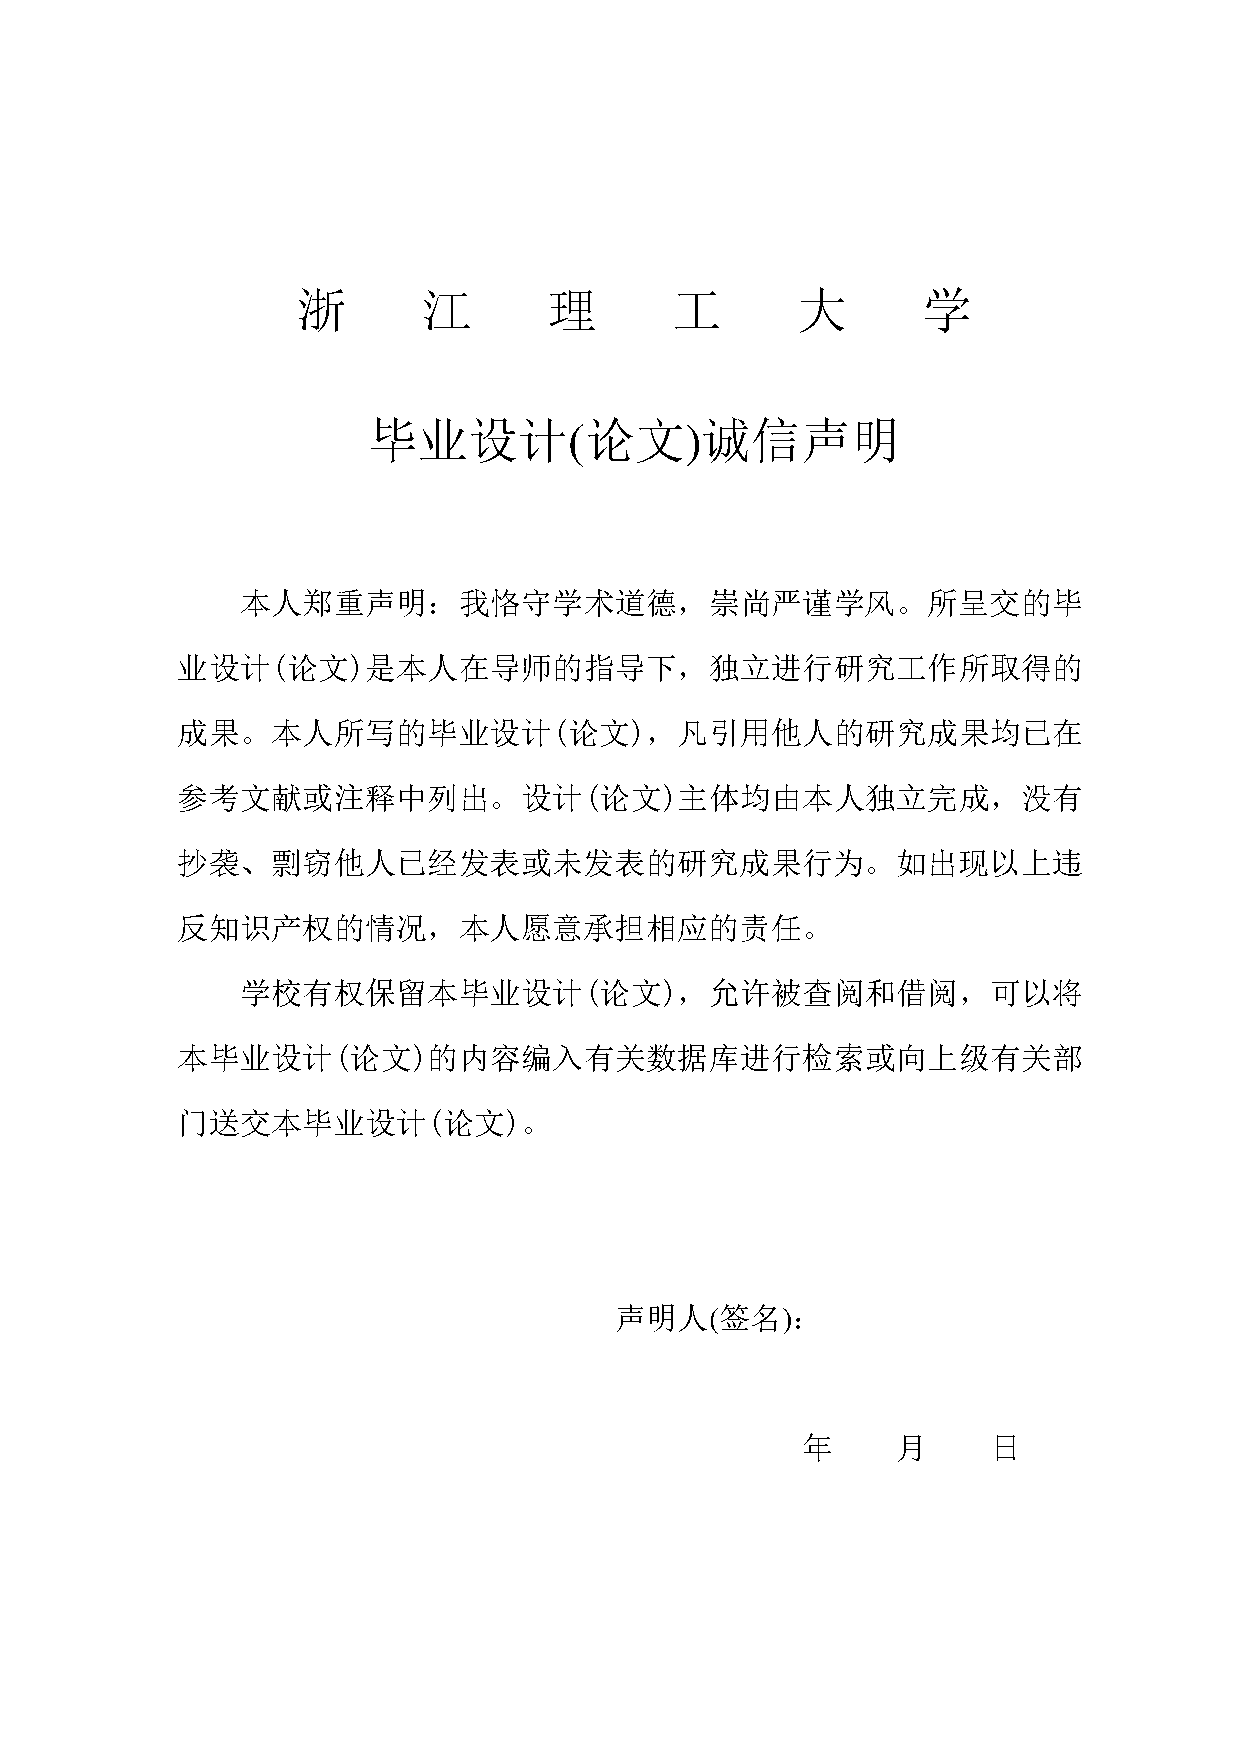
\includepdf[pages=-]{res/诚信声明.pdf}
\myemptypage
% 摘要
\abstractzh{
	随着我国汽车保有量持续增长,城市化进程加速,地面停车资源日益紧张。为解决停车难题,地下停车场被认为是一种有效的解决方案。然而,地库设计与建设依然面临多重挑战,如规范不统一、设计参数繁多、结构复杂等。由于人工设计效率低下,且难以充分利用空地,因此亟需一种能够减轻设计压力、高效利用空地的车位自动化排布算法,同时,能够向设计师提供多种方案参考,并降低图纸设计、修改成本。

	针对以上问题,本文提出了一种基于智能体行为导向和PER-D3QN的车位排布算法。首先,根据障碍物等条件确定地库边界,将图纸栅格化,并在状态矩阵中初始化各地块状态。其次,根据智能体的行为和位置,设计了一种创新的车位布局方法,考虑了排布过程中障碍物、柱网等的影响。随后,本文构建了一个基于PER-D3QN的强化学习模型,其中状态空间由智能体为中心的状态矩阵、智能体距离障碍、车位、边界的信息以及智能体朝向组成,行动空间定义为前进、左转和右转。模型通过数据初始化、特征提取网络、特征融合网络、增强探索性的噪声网络以及决斗网络输出每个行为的预期回报(Q值)。为了更有效地利用有限的数据,本文使用PER算法根据数据优先级进行多次利用。最后,为了评估道路铺设和车位排布效果,本文设计了一个奖励评价系统,主要从车辆和交通两个方面考虑,其中交通包含直路奖励、道路过宽惩罚和重复铺设惩罚。为了验证算法有效性,本文使用了6张不同的标准CAD工程图纸对比了现有算法和本文算法,发现本文提出的算法在处理大规模和复杂障碍的图纸时表现优异,能够在有限空间内最大化车位数量,同时考虑全局和局部信息,得到更优的布局。
}
{
	地下停车场;车位排布;D3QN;PER;智能体行为导向
}

\abstracten{
	As the number of automobiles in China continues to increase and urbanization accelerates, the shortage of surface parking resources becomes increasingly severe. Underground parking lots are considered an effective solution to alleviate this parking problem. However, the design and construction of underground garages still face multiple challenges, such as inconsistent regulations, numerous design parameters, and complex structures. Given the inefficiency of manual design and challenges in space utilization, there's a pressing demand for an automated parking layout algorithm. It should alleviate design pressure, optimize space, offer diverse design options, and cut down on drawing costs and modifications.

	In response to these issues, this paper proposes a parking layout algorithm based on agent behavior guidance and PER-D3QN. Firstly, determine the boundaries of the underground garage based on obstacles and other conditions, gridify the drawings, and initialize the status of each grid block in the state matrix. Secondly, an innovative parking layout method is designed based on the behavior and position of agent, considering the influence of obstacles and columns during the layout process. Thirdly, a reinforcement learning model based on PER-D3QN is constructed, where the state space consists of information such as the state matrix centered on the agent, the distance from obstacles, parking spaces, and boundaries, as well as the orientation of the agent, and the action space is defined as forward, left turn, and right turn. The model outputs the expected return (Q-value) for each action through data initialization, feature extraction network, feature fusion network, enhanced exploratory noise network, and duel network. To more effectively utilize limited data, the PER algorithm is used for multiple exploits based on data priority. Finally, to evaluate the effectiveness of road paving and parking layout, a reward evaluation system is designed, mainly considering vehicles and traffic, where traffic includes rewards for straight roads, penalties for excessively wide roads and redundant paving. To validate the effectiveness of the algorithm, this paper compared the existing algorithm with the proposed one using six different standard CAD engineering drawings. It was found that the algorithm proposed in this paper performs excellently when dealing with large-scale and complex obstacle layouts, maximizing the number of parking spaces within limited space. Additionally, it takes into account both global and local information to achieve optimal layouts.
}
{
	Underground Parking Lot; Parking Space Arrangement; D3QN; PER; Agent Behavior Guidance
}
\myemptypage
% 目录
\maketoc
\myemptypage

% 正文
\section{绪论}
\subsection{选题背景}
随着我国经济社会的快速发展,人们的生活水平显著提高,汽车保有量的持续呈现增长趋势。据中国汽车工业协会数据显示,2023年汽车产销分别完成3016.1万辆和3009.4万辆,同比分别增长11.6\%和12\% ,如图~\ref{fig:cars_sales} 所示。这表明汽车在我国的普及和使用呈现出强劲的发展态势。
\begin{figure}[!htb]
  \centering
  \includesvg[width=0.7\linewidth]{1/汽车销量}
  \caption{\label{fig:cars_sales}2022-2023年中国汽车销量及增长率\\(数据来源:中国汽车工业协会)}
\end{figure}

随着城镇化进程加速\cite{XXCZ202306017},城市密度激增\cite{JZXB201004006},土地资源紧缺问题逐渐凸显。而在这种情况下,人们对于汽车的购买欲望提升,车辆的增加虽然带来了便捷的生活,但也造成了交通系统压力大、停车基础设施不足等问题\cite{CSDQ200708009},如何充分利用停车资源、开发地下停车场\cite{JSSD201905002}并增加经济效益等成为当前城市发展的紧迫问题。

其中,建造地下停车场是一种极为有效的解决方案。同等土地面积下,相较于传统的露天停车场,地下停车场能够提供更多的停车位\cite{1022811825.nh},同时也能节省城市建设用地。此外,地下车库还能有效地缓解地面动静态交通矛盾\cite{CSDQ201807120}。虽然地下车库有诸多优点,但仍存在以下问题:
\begin{enumerate}
  \item 规范不统一。各个公司均用私有规范,导致产生行业壁垒,行业无法快速进步。
  \item 设计参数多。除去政策、法律等规定的固定参数\cite{ZGBZ202119043},还包含了一些不容建筑公司定制化的可变参数。
  \item 结构复杂。相较于地上停车场,地下停车场结构更为复杂。
\end{enumerate}

以上原因,均加剧了地下车库设计远远落后于地上的情况。

在大量建设地下停车场的同时,由于设计师的设计流程较为耗时,未能满足开发商对于周期、质量等的成本要求,因此他们将目光转移到了“一键式”生成设计图。与此同时,Autodesk\cite{carrasco2005innovative,JCJG202304039}等公司开发了一款适用于建筑行业的设计软件AutoCAD,为设计师进行图纸修改提供了更便捷的方式。

基于以上背景,本文致力于设计和开发基于机器学习的车位自动化排布算法并进行可视化展示。
\subsection{选题意义}
\subsubsection{现实意义}
  \paragraph{减轻设计压力} 大幅缩短设计师的设计流程,简化一些较为简单的设计,减少低效的重复劳作。
  \paragraph{提供多种方案} 针对同一初始场地,可利用不同算法进行设计,可能会出现不同的排布方案,便于设计师进行选择。
  \paragraph{降低修改成本} 面对一些特殊情况,如需求改变、车位尺寸改变等,只需付出较少的成本便可重新设计和布局。
\subsubsection{技术意义}
  \paragraph{跨学科融合} 通过将一个较为复杂的地库设计问题转化为计算机可以解决的问题,探究如何将计算机和建筑学进行有机融合,推动计算机辅助设计的进一步发展。

\subsection{非技术因素分析}
非技术因素直接关系到解决方案的实际应用和社会影响。针对本项目提出的基于智能体行为导向和PER-D3QN的车位排布算法,需考虑以下的非技术因素:
\begin{enumerate}
  \item 社会效益: 本项目有望为城市交通管理和城市规划带来积极的影响。通过提高地库设计效率和灵活性,可以更好地满足城市居民和企业的停车需求,缓解城市交通拥堵问题,提升城市交通运行效率,提高城市生活质量。
  \item 经济效益: 地库的建设和管理是一项巨大的经济投资,因此,提高设计效率和降低设计成本对于开发商和设计方都具有重要意义。这项解决方案有望降低地库建设的成本,并提高停车场的利用率,从而提升经济效益。
   \item 环境影响: 地库的建设可能会对周边环境产生一定的影响,如土地利用、地下水位、地质结构等方面。因此,在设计和建设过程中需要充分考虑环境保护和生态平衡,采取相应的环境保护措施,减少对周边环境的影响。
  \item 法律风险: 地库的设计和建设涉及到一系列法律法规和政策规定,包括城市规划、建筑设计、土地利用等方面的法律法规。因此,解决方案的实施需要充分遵守相关法律法规,避免可能存在的法律风险和纠纷。
  \item 社会风险: 地库的设计和建设可能会对周边社区和居民生活产生一定的影响,如噪音、振动、施工期间交通阻塞等。因此,在项目实施过程中需要充分考虑社会影响,采取有效的沟通和协调措施,减少社会风险和负面影响。
\end{enumerate}
  
综上所述,解决方案的实施需要综合考虑各种非技术因素,确保能够最大程度地实现社会、经济和环境效益,同时尽量减少法律和社会风险。
\subsection{国内外研究现状与分析}
\subsubsection{国内外研究现状}
1981年时,Fowler\cite{fowler1981optimal}等人证明无约束的平面布局优化问题是NP完全问题,而将地下车位排布可被看作是带空洞的不规则边界布局优化问题。

针对类似矩阵的地下车库,Birgin\cite{birgin2006method, birgin2006orthogonal}等人提出了通过获取哨兵集,利用非线性规划,实现凸区域内的非重叠打包,并在2010年进一步改进\cite{birgin2010orthogonal},使得矩阵可自由旋转。Cassioli\cite{cassioli2010heuristic}等人结合扰动运动和连续扰动,解决凸区域内等矩形填充问题。L{\'o}pez \cite{lopez2018packing}等人提出利用混合整数非线性规划模型解决圆形容器中的排布问题。

而不同于排布,停车位的设计中还需考虑道路相关信息,例如连通性等。Young、Mendat\cite{young1988review, mendat2003perceptions}等人提出了各种影响停车场需求高效设计的指标。而对于车位排布问题也有着一定的研究,Abdelfatah\cite{abdelfatah2014parking}等人利用整数线性规划(ILP)确定最佳停车角度,并适用于不同环境。Syahrini\cite{syahrini2018mathematical}等人应用整数线性规划优化等腰和等边三角形停车场模型。Hasbiyati\cite{hasbiyati2019parking}等人提出了一种平行四边形形式的停车场的排布,其中平行四边形看作为两个三角形的组合来进行计算。Stephan\cite{stephan2021layout}等人探讨了不同分辨率的正交停车混合整数程序与计算量权衡。

有部分研究进一步考虑停车场的障碍、道路、出入口等因素,并将障碍群成为空洞。Huang\cite{huang2020general}等人研究了基于贪婪算法的单双边停车通道布局选择。利润\cite{1021546706.nh}利用网格分割与满足全局约束的贪婪分割应用于多个排布场景。Guo\cite{guo2022optimal}等人利用非线性规划和模糊评判,解决多形状、多入口、多角度车位的停车场问题。

随着机器学习算法的普及,专家逐渐将排布与机器学习算法结合。Xu\cite{xu2007particle}提出了基于粒子群的算法优化圆形容器内矩形物体布局,并在2010年\cite{xu2010genetic}进一步引入有序定位技术和遗传算法均优化了性能。Cassioli\cite{cassioli2010heuristic}提出启发式方法,通过迭代局部搜索和扰动移动解决矩形填充问题。Zhao\cite{zhao2014human}引入人机协作免疫算法,结合PSO和IA解决布局设计问题。马莹\cite{JSGG201820015}等人提出了自适应量子遗传算法,旨在优化问题求解,并提高材料利用率。Nourinejad\cite{nourinejad2018designing}等人,基于排队路构建了混合整数模型,设计了一种启发式算法,利用Benders进行分解。Chen\cite{chen2022arrangement}等人利用遗传算法优化地下车库标准与非标准停车位布局。

同时,随着自动停车或是自动驾驶车辆的出现,车库也将迎来新的革新。Ferreira\cite{ferreira2014self}等人利用车辆自组织网络和自动技术,优化停车场空间和车辆行驶距离。Timpner\cite{timpner2015k}等人提出自动代客泊车优化模型,显著提高停车密度,减少取车时间,Banzhaf\cite{banzhaf2017high}等人基于前面的优化提出了混合整数规划模型。Kong\cite{kong2018capacity}等人开发混合整数非线性模型,量化自动驾驶对停车效率的影响。Siddique\cite{siddique2021puzzle}等人采用基于谜题和最大密度的设计的方法,求解小型停车场的最佳排布结果,并利用用启发式算法求解大型停车场的排布方式。郑聪\cite{TMJZ202104021}等人基于Dynamo可视化编程,通过模拟设计思路进行自动排布车位。

现仍存在大部分的车库轮廓并非规则,且通常有不规则障碍排布,同时,自动驾驶车辆未普及等问题,专家逐渐转向增加更多的限制条件。徐涵喆\cite{1020726891.nh}通过将图纸分为内圈和外圈,并分别使用遗传算法和贪婪算法进行排布,提高了车库的利用率。黄逸彬等人\cite{BJYD202004002}构建了一种基于图形分割方法的混合整数线性规划模型。冯嘉宇\cite{1022674189.nh}采用像素分割和遗传算法,优化内外圈区域的车位排列。

而随着强化学习的兴起,专家也将注意转移到了基于强化学习的地库排布。余光鑫\cite{1020332216.nh}研究了一种针对规则边缘的基于强化学习的地下停车场生成设计策略,通过边铺设道路,边放置车位的方式,使用简单网络结构和进化策略,但时间开销大,无法对不规则场地进行学习。王潇霆\cite{1022674189.nh}则是改进了强化学习内容,通过每走一步就给予奖励,使得智能体只学习如何铺设道路,但奖励非连续,可解释性较差。

\subsubsection{存在问题及分析}
通过对国内外车位自动化排布已有的研究和参考文献进行分析,发现仍存在如下问题:
\begin{enumerate}
  \item 局限性的奖励机制:现有方法主要依赖固定位置搭配的理论分析来确定具体的奖励值,未充分利用周围所有信息进行计算。  
  \item 过度依赖人工干预:需要对图纸进行区域划分和分别处理,缺乏自动化处理的方法。同时,车位铺设依赖于人工设计,缺乏自动化设计的方法。  
  \item 缺乏实际应用强化学习算法的研究:尽管部分研究借鉴了强化学习的思想,但并未实际运用诸如DQN等强化学习算法进行实践。
  \item 出入口位置的后定问题:现有的研究通常先铺路再放置车位,再设置出入口,但实际情况中,出入口位置需由外界交通决定,且通常位于较为中心的位置,这可能导致设计的实用性不强。
  \end{enumerate}

\subsection{研究目标}
为了缓解停车位供应紧张的问题,本研究的主要目标是在满足建筑规范的条件下,尽可能多地增加车位数量。

\subsection{论文结构安排}
本文共分为六个章节,核心为基于智能体行为导向的车位布局算法、基于PER-D3QN的道路铺设算法、实验例证,具体章节结构安排如图~\ref{fig:chapter_structure}。

第一章主要介绍了地库车位排布自动化的背景及意义,国内外近年来的研究、遇到的问题以及论文结构。

第二章主要介绍了文中涉及的地库排布基础知识和主要应用的技术、算法、模型等。

第三章主要介绍了模型的构建方式,将图纸根据一定精度进行划分,同时介绍了车位铺设的方式。通过道路铺设中智能体的朝向和行为,根据周边的障碍情况,判断车位放置的方向、个数与柱网放置。

第四章主要介绍了基于PER-D3QN的道路铺设算法,将图中信息整合输入到网络中,设定合理奖励,根据总奖励对比同一图不同策略的优越性。

第五章主要介绍了模型中的超参数,与王的研究进行比较并展示不同图纸的绘制情况。

第六章主要归纳了本文的主要工作和成果,指出了研究中的不足,并提出未来研究方向和建议。
\begin{figure}[!htb]
  \centering
  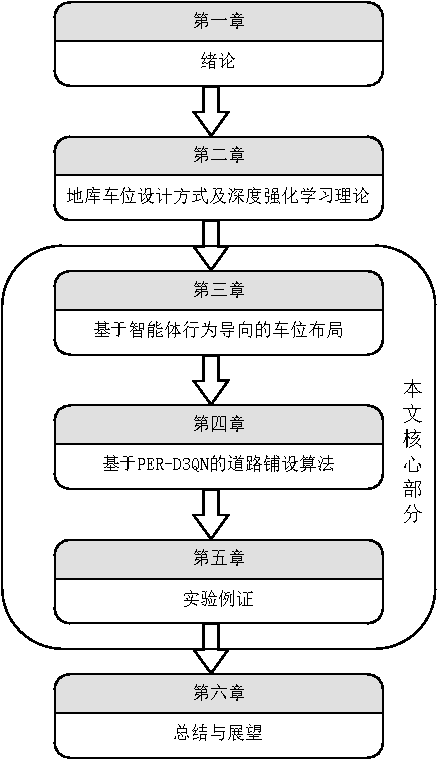
\includegraphics[width=0.75\textwidth]{1/章节结构}
  \caption{论文结构示意图}
  \label{fig:chapter_structure}
\end{figure}
\section{地库车位设计方式及深度强化学习理论}
\subsection{地库设计理论}
\subsubsection{地库设计要点}
地库设计的要点包括但不限于以下几个方面:
\begin{enumerate}
    \item 车位数量规划:地库设计需充分考虑实际需求确定车位数量,尽可能多地提供车位,以确保最佳的车位利用率和通行便利性。
    \item 车位排列方式:地库设计可采用多种排列方式,包括横排、${30}^\circ$、${45}^\circ$、${60}^\circ$和竖排等,以满足不同场地和需求条件下的停车需求。
    \item 车位尺寸及道路设计: 地下停车场的车位尺寸和道路设计应统一规格,符合国家标准和规范要求,确保车辆安全通行和便捷停放,以实现最佳的停车效率、通行安全性和舒适性。
    \item 出入口设置:地库的出入口应设置合理,便于车辆的进出和行人的通行,同时要考虑交通流量和安全性。
    \item 承重柱布局:地下停车场的承重柱应科学布局,以支撑结构并确保地下停车场的安全性。
    \item 安全设施配置:地下停车场的设计应考虑包括消防通道、安全出口和灭火器等设施的配置,以应对紧急情况,确保人员安全疏散和火灾等突发事件的应对能力。
\end{enumerate}
\subsubsection{柱网设置}
在地库设计中,柱网的设置是至关重要的一环,它直接关系到停车场的结构稳定性、通行便利性以及车辆与构筑物之间的净距。柱网是由多个承重柱组成的支撑结构,用于支撑停车场的天花板和地面,并确保停车场的安全运行。
\begin{enumerate}
    \item 柱距间净距要求: 车辆与车辆之间、车辆与构筑物之间的净距应符合相关规定,以确保车辆的安全通行和空间利用。根据规定,地下车库柱距间停放1辆、2辆或3辆汽车时所需的最小柱距分别为3.1米、5.6米和8.1米。
    \item 承重柱布局: 承重柱的布局应合理规划,均匀分布于停车场各个区域,并具备足够的强度和稳定性以支撑停车场结构。
    \item 施工和验收: 施工过程中需严格按设计要求和规范进行操作,确保承重柱的布局、尺寸和材料符合标准。完成后需进行质量检查和验收,确保柱网的稳定性和安全性符合设计要求。
\end{enumerate}

考虑到具体的方案落地情况,柱网间距、车位面积以及通道间隔之间存在着密切的关系,彼此相互制约,直接影响着最终的车位数量和停车场的整体效果。
\subsubsection{车位排列方式}
在地库排布中,为了提高设计的灵活性和高效性,本文引入了车位模块\cite{1020726891.nh}这一概念。车位模块是指一个矩形区域,内部仅能容纳同排列类型车位,并根据一定规律进行摆放。其中主要包含水平、30°、45°、60°和垂直等,如图~\ref{fig:car_paving}。车位模块的引入可以简化地库设计的复杂度,提高设计的灵活性和可扩展性,同时也有利于后续的优化和调整。
\begin{figure}[!htb]
	\centering  
	\subfigure[${45}^\circ$排布]{
		\includesvg[width=0.365\linewidth]{./2/排列45}}
	\subfigure[${30}^\circ$排布]{
		\includesvg[width=0.555\linewidth]{./2/排列30}}
	  \\
	\subfigure[竖直排布]{
		\includesvg[width=0.266\linewidth]{./2/排列垂直}}
	%\quad
	\subfigure[${60}^\circ$排布]{
		\includesvg[width=0.301\linewidth]{./2/排列60}}
	\subfigure[水平排布]{
		\includesvg[width=0.313\linewidth]{./2/排列横向}}
	\caption{车位排列方式}
    \label{fig:car_paving}
\end{figure}

根据图示计算当均容纳六车位时,各类型车位模块长宽:
\begin{equation}
    sqaure_{90^\circ} = (3625,250) 
\end{equation}
\begin{equation}
    sqaure_{60^\circ} = (300 + \frac{3475}{3}\sqrt{3},300\sqrt{3}+125) 
\end{equation}
\begin{equation}
    sqaure_{45^\circ} = (1700\sqrt{2}, 425\sqrt{2})
\end{equation}
\begin{equation}
    sqaure_{30^\circ} = (300\sqrt{3}+3175,300+125\sqrt{3}) 
\end{equation}
\begin{equation}
    sqaure_{0^\circ} = (3725,250)
\end{equation}
其模块总面积大小排序为:$sqaure_{90^\circ}<sqaure_{0^\circ}<sqaure_{45^\circ}<sqaure_{60^\circ}<sqaure_{30^\circ}$。

在本项目中,选择角度为0°和90°的车位模块进行排放,主要有以下原因:

\begin{enumerate}
\item 灵活性和空间利用率:0°和90°的车位模块可以根据地库的形状、尺寸、出入口位置、承重柱位置等因素进行调整,以实现最佳的空间利用率和停车容量。
\item 安全性和便捷性:这两种排放方式使得车位和车道之间排列紧凑、整齐,便于承重柱的设置,确保车辆安全通行和停放,便于进出。
\end{enumerate}

在0°和90°之间,我们优先选择90°的车位模块进行排放,原因如下:

\begin{enumerate}
\item 更高的空间利用率和停车容量:90°车位模块在同样的面积内能够提供更多的停车位。
\item 进出便利性:90°车位模块便于驾驶员操作,提高停车效率。
\item 适应性:90°车位模块更好地配合承重柱布局,减少难以利用的空间。
\end{enumerate}

\subsection{深度强化学习理论}
\subsubsection{强化学习}
强化学习是一种机器学习方法,通过智能体和环境间的不断交互,学习最佳的行为策略。\cite{sutton2018reinforcement}与监督学习和无监督学习不同,强化学习中的反馈是交互产生的,而并非使用预先标记的数据。这种交互过程可以形式化地描述为马尔可夫决策过程(MDP),其中主要包含智能体、环境、状态、行为、策略、奖励等。
\begin{figure}[!htb]
    \centering
    \includesvg[width=0.7\textwidth]{2/强化学习}
    \caption{强化学习示意图}
    \label{fig:rl_structure}
\end{figure}

在图~\ref{fig:rl_structure} 所示的强化学习示意图中,智能体与环境交互,智能体根据环境状态和奖励更新策略,以最大化累积奖励。

通常,强化学习可以被分为两大类别。其中,基于值函数的强化学习侧重于学习状态或状态-行为对的价值,以间接确定最优策略;而基于策略的强化学习则直接学习在给定状态下采取的行为,以最大化累积奖励。
\subsubsection{马尔可夫决策过程与贝尔曼方程}
马尔可夫决策过程(MDP)描述了强化学习问题的数学框架,它的基础是具有“无记忆性”且随机的马尔可夫过程,且相较于马尔可夫奖励过程,进一步引入了行为这一概念。在 MDP 中,智能体在每个时间步 $t$ 处于某个状态 $s_t$,然后选择行为 $a_t$,环境根据状态和行为的组合给予奖励 $r_{t+1}$,智能体根据奖励和下一个状态 $s_{t+1}$ 更新策略。MDP 可以表示为一个五元组 $(S, A, P, R, \gamma)$,表示为$$P(S_{t+1}=s', R_{t+1}=r|S_t=s, A_t=a) = P_{sa}(s', r).$$

贝尔曼方程(Bellman Equation)是MDP的核心,它描述了状态函数($V$)或行为函数($Q$)之间的递归关系,通过将两者相关联,向智能体提供学习和决策的基础。

对于状态值函数 $V$,贝尔曼方程可以表示为:
\begin{equation}
    V_\pi(s) = \sum_{a \in A} \pi(a|s) ( r(s,a) + \gamma \sum_{s' \in S} P(s'|s,a) V^\pi(s') )
\end{equation}

对于行为值函数 $Q$,贝尔曼方程可以表示为:
\begin{equation}
    Q_\pi(s,a) = r(s,a) + \gamma \sum_{s' \in S} P(s'|s,a) \sum_{a' \in A} \pi(a'|s') Q^\pi(s',a')
\end{equation}

这些方程使智能体能够通过迭代更新值函数来优化其策略,以最大化累积奖励。

\subsubsection{深度强化学习}
深度强化学习是一种结合了深度学习和强化学习的方法\cite{mnih2013playing},旨在解决复杂环境和大型状态空间下的决策问题。\cite{1023788635.nh}其核心思想是利用深度神经网络来近似值函数或策略函数,以应对大型状态空间和连续行为空间的挑战。

在深度强化学习中,典型的基于值函数的方法包括基于深度学习的Deep Q-Network(DQN)和Double DQN,这些算法已成功应用于诸如Atari游戏和机器人控制等领域。而基于策略的方法则包括策略梯度方法,例如确定性策略梯度(DDPG)和TRPO(Trust Region Policy Optimization),这些方法在连续行为空间和高维状态空间的问题上表现出色。

根据强化学习的两大类型,本文选择了其中两个较为主流的算法进行介绍。
\paragraph{DQN算法}
DQN(Deep Q-Network)是将神经网略(neural network)和Q-learning结合,利用深度神经网络来近似值函数(Q值函数)\cite{mnih2013playing},从而实现对复杂环境的学习和决策。其核心思想为以下三个部分:
\begin{itemize}
    \item 经验回放:引入经验回放机制,将智能体与环境交互得到的经验存储在经验回放缓冲区中,并通过随机抽样的方式将这些经验用于训练深度神经网络。这一机制的作用在于减少样本之间的相关性,从而提高训练的稳定性和收敛速度。同时,这也使得DQN算法可以离线(off-line)地从存储的经验中学习,而不需要依赖实时的环境反馈。
    \item 固定目标网络是DQN算法的关键部分之一。它使用两个神经网络来估计状态行为值函数:一个用于选择行为(行为网络),另一个用于评估行为的价值(目标网络)。在训练过程中,目标网络的参数会定期固定一段时间,然后周期性地更新为行为网络的参数。这个步骤的目的是为了稳定训练过程,防止参数的不稳定性影响算法的收敛性。
    \item $\epsilon$-贪心策略:以$\epsilon$的概率随机选择行为,反之选择当前状态下具有最大Q值的行为。这一策略的作用在于在探索和利用之间取得平衡,从而更好地探索环境并学习最优策略。
\end{itemize}

下面是DQN算法的基本流程,同时结合图~\ref{fig:dqn} 进行了图像化展示:
\begin{enumerate}
    \item 初始化深度神经网络的参数。
    \item 与环境交互,根据当前策略选择行为,并观察接收反馈。
    \item 将$(s, a, r, s')$存储在经验回放缓冲区中。
    \item 从经验回放缓冲区中随机抽样一批数据,用于训练深度神经网络。
    \item 更新行为网络的参数,使其逼近Q值函数。
    \item 更新目标网络的参数,使其逼近行为网络的参数。
    \item 重复步骤2~6,直到满足停止条件。
\end{enumerate}
\begin{figure}[!htb]
    \centering
    \includesvg[width=0.7\textwidth]{2/dqn}
    \caption{DQN算法流程图}
    \label{fig:dqn}
\end{figure}

\paragraph{PPO算法}
PPO(Proximal Policy Optimization)是一种基于策略优化的强化学习算法\cite{schulman2017proximal}。它通过在更新策略时引入一个剪切项,保证每次更新的策略变化在一个可控的范围内,从而提高学习的稳定性和收敛速度。其核心思想为以下四个部分:
\begin{itemize}
    \item 近端优化:PPO通过限制每次策略更新的幅度,确保策略变化在一个合理的范围内,从而防止过度更新引发的不稳定性和收敛困难。
    \item 剪切项:PPO引入了一个剪切项,用于限制更新前后策略的KL散度(Kullback-Leibler Divergence),保证更新的策略变化不会过大。
    \item 多步优化:PPO在更新策略时通常使用多步优化,即利用多个时序上连续的样本来计算近似优势函数,提高优化的效率和稳定性。
    \item 并行化:PPO算法具有出色的并行化性能,可以有效地利用多核CPU或分布式计算资源,加速算法的收敛速度和训练效率。
\end{itemize}

下面是PPO算法的基本流程,同时结合图~\ref{fig:ppo} 进行了图像化展示:
\begin{enumerate}
    \item 初始化策略函数的参数。
    \item 与环境交互,根据当前策略选择行为,并观察环境的反馈。
    \item 计算策略函数的梯度,并根据剪切项和近端优化的原则更新策略参数。
    \item 重复步骤2-3,直到满足停止条件。
\end{enumerate}
\begin{figure}[!htb]
    \centering
    \includesvg[width=\textwidth]{2/ppo}
    \caption{PPO算法流程图}
    \label{fig:ppo}
\end{figure}

\subsection{决斗网络}
决斗网络(Dueling Network)是一种深度强化学习架构,它通过分离值函数和优势函数的学习来实现,从而提高学习的效率和稳定性,如图~\ref{fig:duiling_net} 所示。
\begin{figure}[!htb]
    \centering
    \includesvg[width=0.7\linewidth]{2/duiling_net}
    \caption{\label{fig:duiling_net}决斗网络示意图}
\end{figure}

传统的Q-learning直接学习一个行为值函数$Q(s, a)$,但这种方法可能会忽视了一个重要的事实,即在很多情况下,无论采取什么行为,状态的价值都是相同的。因此,行为值函数可进一步分解为状态值函数$V(s)$和优势函数$A(s, a)$。状态值函数表示当前状态的价值,而优势函数用于与其他行为进行比较,计算与其他行为相比的价值。

决斗网络的架构包含两个独立的神经网络,一个用于学习状态值函数,另一个用于学习优势函数。这两个网络共享底层的特征提取层,但有各自的输出层。最后,通过一个特殊的聚合层将这两个网络的输出合并,以得到行为值函数。

决斗网络的优点是,它可以更准确地学习状态值函数和优势函数,从而提高学习的效率和稳定性。此外,由于它可以分别学习状态值函数和优势函数,因此它可以更好地处理那些状态值变化大但优势函数变化小的情况,从而提高智能体的性能。

\subsection{优先级经验回放}
优先级经验回放(Prioritized Experience Replay,简称 PER)改进了传统的经验回放机制。在传统的经验回放中,智能体从其经验池(也称为回放缓冲区)中均匀随机地抽取过去的经验进行学习。然而,这种方法忽略了一些经验可能比其他经验更重要的事实。而优先级经验回放通过为每个经验分配优先级,并根据这些优先级来抽取经验,从而解决了这个问题。

\paragraph{\textbf{SumTree}}
在PER中,SumTree常被用于存储和抽取经验。SumTree是一种特殊的二叉树,其每个节点的值等于其子节点的值之和。叶节点存储经验的优先级(通常为TD误差),非叶节点存储其子节点优先级之和。如图~\ref{fig:sumtree} 所示:
\begin{figure}[!htb]
    \centering
    \includesvg[width=0.5\linewidth]{2/sumtree}
    \caption{\label{fig:sumtree}SumTree示意图}
\end{figure}

经验的抽取过程基于其优先级,优先级总和被分为等量的区间,每个区间内随机选取一个数,然后在SumTree中找到对应的经验。例如,假设抽取3个经验,并按照优先级总和(在此例中为49)分为3个区间:$[0, 16]$, $[16, 32]$, $[32, 49]$。在每个区间内随机选取一个数,然后在SumTree中找到对应的经验,若大于左节点,则向右,并将当前数值减去左节点数值,否则向左,直到找到一个叶节点。

通过这种方式,可在每个区间内进行均匀采样,最后得到3个经验。这样,优先级高的经验就有更高的概率被抽取到。

\paragraph{优先级的更新}
在PER中,经验的优先级是动态更新的,其依据是智能体的学习过程中计算的TD误差。TD误差,即智能体预测的Q值与实际Q值之间的差距,可以用以下公式表示:

\begin{equation}
    TD_{error} = r + \gamma \cdot \max_{a'}Q(s', a') - Q(s, a)
\end{equation}

经验的优先级根据TD误差的大小进行调整,TD误差大的经验优先级提高,反之则降低。在SumTree上更新时,需先找到这个经验对应的叶节点并更新,再递归更新所有包含该叶节点的非叶节点的值。优先级的更新公式如下:

\begin{equation}
    P(i) = |TD_{error}| + \epsilon
\end{equation}

其中,$P(i)$是第$i$个经验的优先级,$|TD_{error}|$是TD误差的绝对值,$\epsilon$是一个很小的正数,用来确保优先级永远不会是0。

通过这种方式可以确保SumTree始终反映了所有经验的最新优先级,从而使得优先级高的经验有更高的概率被抽取到。

\paragraph{重要性采样权重}
在优先级经验回放(PER)中,重要性采样权重(ISW)起到关键作用,它不仅影响经验的选择,也调整学习过程。ISW为每个经验计算一个权重,用于调整学习目标。

ISW的计算公式如下:

\begin{equation}
    ISW(i) = \left( N \cdot P(i) \right)^{-\beta}
\end{equation}

其中,$N$是经验的总数,$P(i)$是第$i$个经验的优先级,$\beta$是一个介于0和1之间的参数,用来控制重要性采样权重的影响程度。

ISW的主要作用是平衡各经验在学习过程中的影响,避免优先级高的经验被过度采样,优先级低的经验被忽视。通过ISW,所有经验都有被学习的机会,从而使得智能体可以从所有的经验中学习。

在实际应用中,每个更新步骤开始时,先计算所有经验的ISW,然后在计算学习目标时使用这些权重,以确保每个更新步骤都考虑到所有经验的优先级。

\subsection{工具选型}
\subsubsection{Pytorch}
PyTorch是一款基于Python的库,以其在科学研究、教育和工业界广泛应用的深度学习框架而闻名。它提供了基于数组的编程模型,通过GPU加速实现微分功能,并与Python生态系统中的自动微分紧密集成。同时,PyTorch自然地与标准绘图、调试和数据处理工具集成,采用命令式编程模型。支持与外部库双向交换数据,用户可以根据项目需求或性能要求自由更换组件。PyTorch实现了张量数据结构、GPU和CPU操作符以及基本的并行原语。它的自动微分系统包括对大多数内置函数的梯度计算,具有立即执行动态张量计算的能力,性能上与当前最快的深度学习库相媲美,在研究社区中备受欢迎(如2019年ICLR提交的296篇论文中提到的\cite{paszke2019pytorch})。

在本项目中,本文选择使用Pytorch实现自定义的深度学习模型,并便捷地处理高维输入输出,同时利用分布式训练在多个GPU上并行训练,为项目实现提供了高效可靠的解决方案。
\subsubsection{pyautocad}
pyautocad\cite{shahzad2023implementing}是一款专注于与AutoCAD软件交互的Python库,通过AutoCAD的COM接口实现对AutoCAD对象模型的访问和操作。具有多版本支持、执行AutoLISP代码的功能,其直观且方便的API设计使得通过Python直接调用AutoCAD的对象和方法变得简便。尤其适用于需要自动化处理CAD图纸的项目,拥有丰富的社区支持和文档资源,为开发人员提供了可靠的工具。

在本项目中,pyautocad通过利用与AutoCAD的强大交互能力,高效地实现对CAD图纸的自动修改和处理,也便于生成后的进一步修改。pyautocad为项目提供了便捷而可靠的解决方案,使得与AutoCAD集成的开发变得更加顺畅。
\subsubsection{AutoCAD}
AutoCAD是由AutoDesk公司开发的计算机辅助设计(CAD)软件,广泛应用于建筑和土木工程等领域。它提供了强大的绘图和建模工具,可用于创建、编辑和分析二、三维设计。其用户友好的界面和丰富的功能集使得设计师能够高效地进行各种设计任务,从简单的图纸绘制到复杂的建筑模型。

在该项目中,AutoCAD提供了强大的绘图和建模工具,通过对于绘制在AutoCAD中图纸,使得设计师能够轻松编辑并更改生成后的图纸。其支持DWG格式的特性也确保了设计图的广泛可用性。此外,AutoCAD的灵活性和可扩展性使其能够与其他工具和编程语言进行集成,如通过pyautocad连接Python脚本,实现与算法代码的交互。这种整合为项目提供了便捷的工具,使得设计和修改车库布局更加直观、高效。AutoCAD在车库设计项目中的应用为设计师提供了一个全面的平台,满足各种设计需求,从而提高了设计效率和质量。
\section{基于智能体行为导向的车位布局}
\subsection{地库环境构建}
\subsubsection{问题描述}
地库排布问题的输入为CAD图纸,但由于图纸情况较为复杂,存在着斜边、障碍等,同时道路、车位、柱网等尺寸都不相同,因此需要简化图纸,便于后续处理。本文将按照如下步骤进行地库环境矩阵化:
\begin{enumerate}
    \item 首先,根据给定的边界内部点,确定地库边界,其中,包含该点的最大多边形区域记为$S_{boundary}$。
    \item 其次,遍历获取图中的障碍块$S_{bar}=\{S_{bar}^{j}|j\in \{1,2,\dots,n_{bar}\}\}$与其对应的建筑集$S_{build}^{j}=\{S_{build_i}^{j}|j\in \{1,2,\dots,n_{build}\}\}$,以及出入口$S_{ent}=\{S_{ent}^{j}|j\in \{1,2,\dots,n_{ent}\}\}$,其中$\forall S_{build_i}^{j} \subseteq S_{bar}^{j}$。
    \item 接着,根据当前坐标轴,寻找$S_{boundary}$的轴对齐外接矩形$S_{rec}$,其平行于x轴长度为$length_x$,平行于y轴长度为$length_y$。并以$\mu = 0.50m$的精度\cite{1023719817.nh}对$S_{rec}$、$S_{bar}$、$S_{ent}$进行矩阵化操作,确定了矩阵$S_{rec}$的行列数分别为$m$、$n$,其中$m=\lceil \frac{length_y}{\mu} \rceil$,$n=\lceil \frac{length_x}{\mu} \rceil$,矩阵化结果如图~\ref{fig:matrixization} 所示。
          \begin{figure}[!htb]
              \centering
              \includesvg[width=0.5\textwidth]{3/图纸矩阵化}
              \caption{图纸矩阵化示例图}
              \label{fig:matrixization}
          \end{figure}
    \item 同时,为了初始化$S_{rec}$得到初始状态矩阵$S_{state}^0$,需针对每个地块$S_{cell}^{(i,j)}=\{(x_0,y_0),(x_1,y_1)\}$定义不同的标记,其中$(x_0,y_0)$为该地块左下角坐标,$(x_1,y_1)$为该地块右上角坐标。若地块位于出入口$S_{ent}$区域,则标记为-3;若地块位于边界$S_{border}$区域,则标记为-2;若地块位于障碍区域$S_{bar}$,则标记为-1;若地块已被铺设为道路$S_{road}$,则标记为1;若地块已被放置为车位$S_{car}$,则被标记为2;其余为空地$S_{space}$,标记为0。矩阵$S_{state}$中所有网格的状态标记如公式~\ref{state} 所示,其计算或放置优先级如表~\ref{tab:diff_sqaure} 所示。
          \begin{equation}
              \label{state}
              S_{state}(i,j)=\left\{
              \begin{array}{ll}
                  -3, \quad & S_{cell}^{(i,j)} \in S_{space}  \\
                  -2,       & S_{cell}^{(i,j)} \in S_{border} \\
                  -1,       & S_{cell}^{(i,j)} \in S_{bar}    \\
                  0,        & S_{cell}^{(i,j)} \in S_{space}  \\
                  1,        & S_{cell}^{(i,j)} \in S_{road}   \\
                  2,        & S_{cell}^{(i,j)} \in S_{car}
              \end{array}
              \right.,i \in [0,m), j \in [0,n)
          \end{equation}
          \begin{table}[!htb]
              \caption{不同地块含义及优先级}
              \label{tab:diff_sqaure}
              \centering
              \linespread{1.25}\selectfont
              % 调整表格缩放
              \begin{tabular}{C{1cm} C{1.5cm} C{1.5cm}}
                  \hline
                  标记 & 含义  & 优先级 \\
                  \hline
                  -3 & 出入口 & 3   \\
                  -2 & 边界  & 1   \\
                  -1 & 障碍  & 2   \\
                  0  & 空地  & 5   \\
                  1  & 道路  & 4   \\
                  2  & 车位  & 6   \\
                  \hline
                  
              \end{tabular}
              % \caption{(a)不同地块含义及其优先级(b)状态矩阵示例图}
          \end{table}
    \item 完成以上初始化后,智能体便于该图中边铺设道路,边放置车位。最终生成的状态矩阵$S_{state}^n$如图~\ref{fig:matrix_exam} 所示。
          \begin{figure}[!htb]
              \centering
              \includesvg[width=0.5\textwidth]{3/状态矩阵示例图}
              \caption{状态矩阵示例图}
              \label{fig:matrix_exam}
          \end{figure}
\end{enumerate}
\subsubsection{约束条件}
在地库车位排布问题中,主体部分包括道路$R=\{R_k|k=\{1,2,\dots,n_{road}\}\}$、车位$P_m=\{P_m^k|k=\{1,2,\dots,n_{car}\}\}$、障碍$S_{bar}$,本文主要考虑以下三个约束条件:
\paragraph{内在约束}确保道路的连通性和车位间的独立性。
\begin{itemize}
    \item 道路:为保证道路的连通性,算法中的智能体会向相邻网格移动,从而确保道路构成一个连通图。
    \item 车位:为精确记录车位的位置,本文使用具体的车位坐标进行存储,即$P_m^k=\{(x_0,y_0),(x_1,y_1)\}$,其中$(x_0,y_0)$为车位的左下角坐标,$(x_1,y_1)$为车位的右上角坐标。在$S_{state}$中,为了便于后续处理,本文需要对每个车位进行网络切割并标记。为确保车位的有效使用,车位间不能重叠,即$$\forall P_m^i,P_m^j \in P_m,i \neq j,P_m^i \cap P_m^j = \varnothing,$$车位只可相邻排布,既保证了足够的停放空间,又确保交通流畅。
\end{itemize}
\paragraph{交叉约束}
道路、障碍和车位两两互不相交。
\begin{itemize}
    \item 道路与障碍:需保证道路不被障碍遮挡,即$$\forall S_{bar}^i \in S_{bar},\forall R_j \in R,S_{bar}^i \cap R_j.$$
    \item 道路与车位:为同时保证道路和车位的空间占用,需避免两者重合,即$$\forall P_m^i \in P_m,\forall R_j \in R,P_m^i \cap R_j.$$
    \item 障碍与车位:为保证车位尺寸达到标准,需保证放置位置不与障碍重合,即$$\forall P_m^i \in P_m,\forall S_{bar}^j \in S_{bar},P_m^i \cap S_{bar}^j.$$
\end{itemize}
\paragraph{包含约束}
为保证道路、障碍和车位的有效性,需保证其均位于边界内,即$$\forall R_j \in R,\forall S_{bar}^i \in S_{bar},\forall P_m^k \in P_m,R_j \cup S_{bar}^i \cup P_m^k \subseteq S_{boundary}.$$
% 训练集相当于经验池
\subsection{智能体行为导向的车位排布算法}
在地库排布问题中,智能体仅需要进行道路铺设任务,根据当前智能体铺设道路时的朝向、行为和位置,判断当前道路周围应如何放置车位。

\subsubsection{车位铺设方向选择}
智能体的大致行为可以分为直行和转弯两种,其中直行行为是指智能体在当前位置沿着当前方向直行,转弯行为是指智能体在当前位置转向。

若是直行,则只需在道路两侧铺设,如图~\ref{fig:stri_pave},若是转向,则需在道路外侧铺路,如图~\ref{fig:turn_pave}。
\begin{figure}[!htb]
    \centering
	\subfigure[\label{fig:stri_pave}车位直行铺设]{
		\includesvg[width=0.32\linewidth]{3/直行铺设}}\hspace{2cm}
	\subfigure[\label{fig:turn_pave}车位转向铺设]{
		\includesvg[width=0.26\linewidth]{3/转向铺设}}
    \caption{车位铺设示意图}
\end{figure}

\subsubsection{无障碍的车位布局}
\label{section:no_obstacle}
在无障碍的情况下,可进行更自由地布置车位。具体来说,先向道路两侧拓展一个车位宽和道路长的矩形区域,然后在这个区域内布置车位。
\paragraph{直行放置}
在直行铺设车位时,从当前道路两侧的基础排布点开始计算,如图~\ref{fig:stri_pave_pro} 所示。其中,图~\ref{fig:stri_pave_pro}~\subref{fig:stri_pave_1} 展示了铺设前车位放置的情况,图~\ref{fig:stri_pave_pro}~\subref{fig:stri_pave_2} 展示了当前步在待铺设区域内铺设车位后的情况。
\begin{figure}[!htb]
    \centering
	\subfigure[\label{fig:stri_pave_1}铺设前车位放置状况]{
		\includesvg[width=0.4\linewidth]{3/无障碍直行铺路1}}\hspace{1cm}
	\subfigure[\label{fig:stri_pave_2}铺设后车位放置情况]{
		\includesvg[width=0.4\linewidth]{3/无障碍直行铺路2}}
    \caption{\label{fig:stri_pave_pro}无障碍直行铺路过程}
\end{figure}

\paragraph{转向放置}
在转向铺设车位时,向需铺设的边拓展一个车位宽和道路长的矩形区域,也同样从基础排布点开始计算车位的位置,如图~\ref{fig:turn_pave_pro} 所示。其中,图~\ref{fig:turn_pave_pro}~\subref{fig:turn_pave_1} 展示了铺设前车位放置的情况。铺设总体分为两步,第一步铺设转向前外侧区域,并在铺设完成后重置转向后的两侧道路初始排布位置,其中内侧取决于上一边最后的车位,外侧则取决于转弯点,如图~\ref{fig:turn_pave_pro}~\subref{fig:turn_pave_2} 所示;第二步铺设转后前外侧区域,如图~\ref{fig:turn_pave_pro}~\subref{fig:turn_pave_3} 所示。
\begin{figure}[!htb]
    \centering
	\subfigure[\label{fig:turn_pave_1}铺设前车位放置状况]{
		\includesvg[width=0.42\linewidth]{3/无障碍转向铺路1}}
	\subfigure[\label{fig:turn_pave_2}转向前外侧车位放置情况及基础排布点设置]{
		\includesvg[width=0.4\linewidth]{3/无障碍转向铺路2}}\\
	\subfigure[\label{fig:turn_pave_3}转向后外侧车位放置情况及基础排布点设置]{
		\includesvg[width=0.42\linewidth]{3/无障碍转向铺路3}}
    \caption{\label{fig:turn_pave_pro}无障碍转向铺路过程}
\end{figure}

\subsubsection{有障碍的车位布局}
在有障碍的情况下,便有更多的限制因素,以避免与障碍物发生冲突。具体来说,需要根据障碍物到道路的距离,以及车辆的宽度和长度,来确定车位的布置方式。
\paragraph{直行放置}
在直行铺设车位时,本文将情况归纳为以下3种,如图~\ref{fig:stri_obstacle} 所示。记障碍物到道路的距离为$d$,车辆宽度为$car_{width}$,车辆长度为$car_{length}$。若$d<car_{width}$,则无法容纳任何车辆,该区域作废,从障碍的另一侧开始放置;若$d<car_{length}$,则可容纳横向车位,即平行于道路,在障碍和道路之间沿道路铺设横向车位;若$d\geq car_{length}$,则表示向外拓展的区域内无障碍,与\ref{section:no_obstacle}直行铺设中情况相同,则可正常铺设纵向车位,即垂直于道路。其中,此处的障碍物包含边界、障碍和车位。
\begin{figure}[!htb]
    \centering
	\subfigure[\label{fig:dis_lt_cw}距离小于车位宽度]{
		\includesvg[width=0.32\linewidth]{3/距离小于车位宽}}\hspace{1cm}
	\subfigure[\label{fig:dis_lt_cl}距离小于车位长度]{
		\includesvg[width=0.34\linewidth]{3/距离小于车位长}}\\
	\subfigure[\label{fig:dis_gt_cl}距离大于等于车位长度]{
		\includesvg[width=0.38\linewidth]{3/距离大于车位长}}
    \caption{\label{fig:stri_obstacle}不同障碍与道路距离的直行铺设情况}
\end{figure}
\paragraph{转向放置}
在转向铺设车位时,本文需要特别注意内侧有障碍物的情况。如图~\ref{fig:turn_obstacle} 所示,与\ref{section:no_obstacle}转向铺设中情况相似,但在转弯时,如果相较于最后的车位,障碍离转向处更近,则仅在第一步转向前车位放置完毕后有所不同,需将该内侧起始点移至障碍物在智能体转向后的朝向一侧,即图~\ref{fig:turn_pave} 中的障碍物的左侧。
\begin{figure}[!htb]
    \centering
	\subfigure[\label{fig:turn_obstacle_pave_1}铺设前车位放置状况]{
		\includesvg[width=0.4\linewidth]{3/有障碍转向铺路1}}\hspace{1cm}
	\subfigure[\label{fig:turn_obstacle_pave_2}转向前外侧车位放置情况及基础排布点设置]{
		\includesvg[width=0.42\linewidth]{3/有障碍转向铺路2}}\\
	\subfigure[\label{fig:turn_obstacle_pave_3}转向后外侧车位放置情况及基础排布点设置]{
		\includesvg[width=0.42\linewidth]{3/有障碍转向铺路3}}
    \caption{\label{fig:turn_obstacle}有障碍转向铺路过程}
\end{figure}
\subsubsection{柱网的布置}
在设计车位布局时,柱子的位置是一个重要的考虑因素,因为它们对车位的数量和布局有直接影响。如图~\ref{fig:column_pave} 所示,根据车位的朝向,需要添加的柱子的位置会有所不同。对于横向车位,为了保证车辆的安全和方便,至少每三个车位放置一个柱子,如图~\ref{fig:column_pave}~\subref{fig:vertical_parking} 所示。而对于纵向车位,由于空间的限制和车辆的行驶方向,需在每个车位之间都放置一个柱子,如图~\ref{fig:column_pave}~\subref{fig:horizontal_parking} 所示。
\begin{figure}[!htb]
    \centering
	\subfigure[\label{fig:vertical_parking}纵向车位的柱网铺设]{
		\includesvg[width=0.26\linewidth]{3/纵向车位}}
	\subfigure[\label{fig:horizontal_parking}横向车位的柱网铺设]{
		\includesvg[width=0.36\linewidth]{3/横向车位}}
    \caption{\label{fig:column_pave}柱网铺设}
\end{figure}
\paragraph{直行放置}
在直行铺设车位时,需在每条道路两侧,预先放置与行进方向相反侧的柱子,然后再放置车位。这样做的目的是为了确保车位的安全和方便。同时,在放置柱子之前,还需要判断当前是否还可以继续放置车位,以最大化车位的数量。如图~\ref{fig:strai_pillar} 所示,是直行时柱网的放置示意图。
\begin{figure}[!htb]
    \centering
    \subfigure[\label{fig:strai_pillar_possible}未满足最少柱网放置要求]{
        \includesvg[width=0.33\linewidth]{3/竖向车位1}\hspace{2cm}
        \includesvg[width=0.33\linewidth]{3/竖向车位2}}\\
    \subfigure[\label{fig:strai_pillar_impossible}满足最少柱网放置要求]{
        \includesvg[width=0.26\linewidth]{3/竖向车位3}\hspace{2cm}
        \includesvg[width=0.33\linewidth]{3/横向车位1}}
    \caption{\label{fig:strai_pillar}直行时柱网的放置}
\end{figure}
\paragraph{转向放置}
在转向铺设车位时,柱网的放置与直行放置基本相同,但还需额外考虑转向的影响。具体来说,需要判断当前道路最后的车位朝智能体转弯前朝向一侧是否可以放置一个柱子。如果可以,就在放置一个柱子;反之,则将最后一个车位移除,然后再紧接着车位放置一个柱子(若移除后是柱子,则不进行其他操作)。如图~\ref{fig:turn_pillar} 所示,是转向时向街边两侧放柱子的示意图。
\begin{figure}[H]
    \centering
	\subfigure[\label{fig:turn_pillar_possible}转向街边两侧均可放柱子]{
		\includesvg[width=0.3\linewidth]{3/转向可放柱}}\\
	\subfigure[\label{fig:turn_pillar_impossible}转向街边两侧无法放柱子]{
		\includesvg[width=0.3\linewidth]{3/转向不可放柱1}\hspace{1cm}
		\includesvg[width=0.3\linewidth]{3/转向不可放柱2}}
    \caption{\label{fig:turn_pillar}转向时向街边两侧放柱子}
\end{figure}

\section{基于PER-D3QN的道路铺设算法}
为了解决地库车位排布问题,本文使用了深度强化学习中的一种算法——优先经验回放-决斗双重深度Q网络(Prioritized Experience Replay - Dueling Double Deep Q-Network,简称PER-D3QN)。在这个模型中,本文设计了一个神经网络来处理输入的状态信息,并输出各个行为相应的Q值。

在地库车位排布问题中,本文将车位排布的过程抽象为一个强化学习问题。在这个问题中,本文定义了状态空间和行为空间,以及智能体的奖励机制,从而构建了一个完整的强化学习模型。
\subsection{状态空间和行为空间}
在模型中,状态空间和行为空间是两个关键的概念,它们定义了智能体的决策环境和可能的行为。
\subsubsection{状态空间}
状态空间是智能体环境感知的核心,它包含了丰富的环境元素信息,如车位、道路、空地、障碍、边界和出入口等。每个元素都被赋予了一个特定的数值,以表示其在环境中的位置和状态。这种数学表达方式使得复杂的环境信息得以简化,从而方便智能体进行处理和理解。

状态空间主要由三个部分构成:以智能体为中心的$11\times 11$状态矩阵信息、智能体距离四周障碍、车位、边界等的距离信息、以及智能体的朝向信息。这些信息共同构成了智能体的环境感知,为智能体的决策提供了必要的信息。

对于$11\times 11$状态矩阵信息,假设道路宽度为$M$,当前步所在矩阵为$$S_{cur}=\left\{S_{state}^{(o,p)}|m_i\leq o\leq m_i+M, m_j\leq p\leq m_j+M\right\}.$$因此,当前周边状态矩阵信息为$$S_{11aro}=\left\{S_{state}^{(o,p)}|m_i-5M\leq o\leq m_i+6M, m_j-5M\leq p\leq m_j+6M\right\}.$$当框取的矩阵超出边界时,边界外元素也置为边界。其拓展及未拓展情况如图~\ref{fig:11_11} 所示。
\begin{figure}[!htb]
    \centering
    \includesvg[width=0.7\textwidth]{4/11_11_拓展}
    \caption{四周状态矩阵及拓展示意图}
    \label{fig:11_11}
\end{figure}

四周距离信息是通过在环境中向四周遍历得到的,遍历过程会在当前位置为障碍、车位、边界时停止。智能体的朝向信息用于模拟智能体在环境中的行为。

这种状态空间的设计使得智能体能够有效地感知其周围环境,从而做出更加合理和高效的决策。
\subsubsection{行为空间}
行为空间则定义了智能体可以采取的所有行为。在模型中,智能体可以选择向前、向左或向右三个方向进行移动。每个行为都对应了一个特定的行为,例如,向前表示智能体向前移动一步,向左表示智能体向左转向,向右表示智能体向右转向。通过在行为空间中选择不同的行为,智能体可以根据当前的状态信息,做出最优的决策,从而有效地进行车位排布。
\subsection{网络结构}
本文设计了一个由多个主要部分组成的神经网络模型,如图~\ref{fig:network} 所示。该模型通过将周围信息放入状态矩阵信息提取网络,并同四周距离一期放入特征融合网络,最后输出各行为的Q值,以指导智能体进行车位排布。
\begin{figure}[!htb]
    \centering
    \includesvg[width=\textwidth]{4/网络结构}
    \caption{网络结构示意图}
    \label{fig:network}
\end{figure}
\subsubsection{数据初始化}
神经网络的输入由两部分信息组成:一部分是智能体距离四周障碍、车位、边界等的距离信息,另一部分是以智能体为中心的$11\times 11$的状态矩阵信息。状态矩阵包含了智能体周围的环境信息,如车位、道路、障碍物和边界等的位置信息。
\paragraph{视角一致}
为了模拟汽车在实际环境中的视野范围,本文还获取了智能体当前的朝向信息。这样,智能体就可以根据自己的朝向来理解和判断周围的环境,从而更好地进行决策。

在处理输入信息的过程中,本文采用了一种特定的策略以适应智能体的视角,如图~\ref{fig:consistent_perspective} 所示。首先,设定智能体的默认朝向为向上。随后,需将以智能体为中心的$11\times 11$的状态矩阵进行旋转,使得智能体朝向始终保持向上。同样,对距离信息也进行类似的处理,将其调整为相对于智能体朝向的[前,左,后,右]的顺序。
\begin{figure}[!htb]
    \centering
    \includesvg[width=\textwidth]{4/视角一致}
    \caption{视觉一致性示意图}
    \label{fig:consistent_perspective}
\end{figure}

通过这种方式,本文实现了一种视角一致的信息处理方式,使得智能体无论在何种朝向,都能以一致的方式理解其周围的环境。这大大简化了智能体的决策过程,使其能够更有效地进行学习和决策。
\paragraph{独热编码}
在处理状态矩阵时,本文采用了独热编码策略。由于状态矩阵中的元素是离散的,直接输入到神经网络可能会导致模型难以理解其含义。因此,将每个元素转换为一个独热编码向量,这样可以更直观地表示其在环境中的位置和状态,如图~\ref{fig:one_hot} 所示。
\begin{figure}[!htb]
    \centering
    \includesvg[width=\textwidth]{4/独热编码}
    \caption{独热编码示意图}
    \label{fig:one_hot}
\end{figure}

通过这种方式,神经网络模型可以有效地处理和理解输入的状态信息,从而为智能体提供更准确的决策依据。这种处理输入信息的策略,使得模型能够更好地理解和处理复杂的环境信息,从而更好地进行决策。
\subsubsection{特征提取网络}
在神经网络模型中,特征提取是一个关键的步骤。为了从初始化后的数据中提取有用的特征,网络中引入了一个卷积神经网络(Convolutional Neural Network,简称CNN)。首先,通过两个卷积层进行特征提取。每个卷积层都包含了一组卷积核,这些卷积核可以在输入数据上滑动,从而提取出不同的特征。在每个卷积层后连接一个最大池化层,用于降低特征维度,同时保留最重要的信息,在保证减少模型计算复杂度的同时,避免过拟合。

经过卷积和池化操作后,得到了一组二维的特征图。将这些特征图进行平坦化操作,将其转换为一维向量,方便与一维的四周距离信息进行连接,作为后续特征融合网络的输入。

通过这种方式,模型能有效提取状态矩阵中的特征,从而更好地理解和判断智能体的周围环境,为智能体的决策提供更准确的依据。
\subsubsection{特征融合网络}
本文设计了一个特征融合网络,该网络将特征提取网络的输出与四周距离信息进行拼接,使得模型能够同时考虑到智能体的局部环境和全局环境,从而做出更全面的决策。

特征融合网络主要由两个全连接层组成,它们的任务是进一步提取和整合特征。全连接层通过进行线性变换,将融合后的特征转换为新的特征空间,这种转换可以帮助模型学习到更复杂的特征和模式,从而提高模型的性能。本文还在全连接层之后引入了ReLU非线性激活函数,以增加模型的非线性表达能力。这种处理方式使得模型能够更好地理解和判断智能体的周围环境,为智能体的决策提供更准确的依据。

通过这种方式,模型可以有效地处理和理解输入的状态信息,从而为智能体提供更准确的决策依据,进一步提高车位排布的效率和质量。
\subsubsection{噪声网络及输出}
在特征融合后,引入了一个噪声网络层,以增强模型的探索能力。在强化学习中,探索是关键,因为它使模型有可能发现更优的策略。然而,过度的探索可能导致模型训练过程中的不稳定性。为了解决这个问题,本文采用了噪声网络,它在训练过程中向模型的权重和偏置添加参数化噪声,以增强模型的探索性。

噪声网络是一个带有参数化噪声的线性层,它在训练过程中向权重和偏置添加噪声。这种噪声不是固定的,而是作为模型的一部分进行学习和优化。这意味着,随着训练的进行,模型可以学习如何最好地利用这种噪声来增强其探索性,同时保持其性能的稳定性。

在每次前向传播过程中,如果模块处于训练模式,它会重置噪声并将噪声添加到权重和偏置的均值上。如果模块处于评估模式,它将只使用权重和偏置的均值。这种设计使得模型在训练时能够增强探索性,而在评估时保持稳定性。

最后,本文采用了决斗网络架构来进行决策。这种架构能够让模型更准确地估计每个行为的价值。通过这种方式,本文的模型可以有效地处理车位排布问题的状态信息,并输出相应的行为值,从而指导智能体进行有效的车位排布。
\subsection{奖励设计}
在模型中,设计了一个奖励评价体系来评估每一轮算法放置道路的效果。

在强化学习中,奖励与惩罚机制的结合设置至关重要,因为它们协同作用,引导智能体学习最优策略。奖励机制通过正向激励来强化正确行为,帮助智能体识别并重复有助于实现目标的行为,从而提升策略的整体质量。另一方面,惩罚机制通过负向激励来抑制错误行为,促使智能体快速识别并避免低效或有害的行为,加速学习过程的收敛。奖励和惩罚的结合不仅有效地平衡了探索与利用,确保智能体在不同环境中高效学习,还通过规避高风险行为提升了系统的安全性和可靠性。

本文中的奖励评价体系主要包括两个部分:车辆(Car)和交通(Traffic)\cite{zheng2023spatial}。每一步的具体奖励计算公式如下所示:
\begin{equation}
    \label{reward}
    R_i = \alpha_c Car_i + \alpha_t Traffic_i
\end{equation}

交通部分则主要反映了当前的道路铺设情况,包括直路奖励$T_{linearity}$、道路过宽惩罚$T_{space}$和重复铺设惩罚$T_{overlap}$
\begin{equation}
    Traffic_i = \beta_l T_{linearity_i} + \beta_s T_{space_i} + \beta_o T_{overlap_i}
\end{equation}

其中$\alpha_c$、$\alpha_t$、$\beta_l$、$\beta_s$、$\beta_o$为权重参数。

由于状态矩阵中每个元素表示精度大小的方形,当智能体铺设道路时,每一步均为道路宽度大小的方形,因此一步中包含$M\times M$个精度大小的方形。当第$i$步时,其左下角标记点位于第$m_i$行$n_i$列,定义其所在的方格为$B_i$,其中第$k$行$l$列为$$b^{i}_{kl} = S_{state}^{(m_i+m,n_i+n)}.$$

\subsubsection{车辆}
车辆部分主要考虑的是车位数量变化,当第$i$步时,其公式为:
\begin{equation}
    \label{car_num}
    Car_i = \left\{
    \begin{array}{ll}
        Nc_i - Nc_{i-1},\quad & \quad i \geq 2 \\
        0\quad                          & \quad i = 1
    \end{array}
    \right.
\end{equation}

公式中,$Nc_i$表示第$i$步车辆数。当式子返回的值大于0时,表示该步导致车辆数增加,为奖励;当值小于0时,表示该步导致车位减少,变为惩罚;否则车位数不变,不影响。
\subsubsection{交通}
\paragraph{直路奖励}
当智能体在道路上行走时,需要保证道路的连通性,即道路尽量不断裂的情况。为了实现这一目标,本文设计了直路奖励机制,以鼓励智能体铺设连续的道路,如图~\ref{fig:stri_road} 。
\begin{figure}[!htb]
    \centering
    \includesvg[width=0.5\linewidth]{4/直路}
    \caption{\label{fig:stri_road}直路示意图}
\end{figure}

当第$i$步时,奖励为
\begin{equation}
    \begin{aligned}
    T_{linearity_i} = & (U_{i-1}(o,p) \land D_{i-1}(o,p) \land \neg L_{i-1}(o,p) \land \neg R_{i-1}(o,p)) \lor \\ 
    & (\neg U_{i-1}(o,p) \land \neg D_{i-1}(o,p) \land  L_{i-1}(o,p) \land  R_{i-1}(o,p)).
    \end{aligned}
\end{equation}

实际计算中,需考虑上一步的相邻路块中是否全为道路,即从宏观上与相邻路块联通。设$U$、$D$、$L$、$R$为方格$B$的上、下、左、右方格。若对向方向均为道路,则返回1,为奖励;否则,返回0,不影响。
\paragraph{道路过宽惩罚}
道路过宽惩罚主要考虑的是道路的宽度是否超过了预设的最大宽度,如图~\ref{fig:excessive_road} 所示:
\begin{figure}[!htb]
    \centering
    \includesvg[width=0.3\textwidth]{4/道路过宽}
    \caption{道路过宽示例图}
    \label{fig:excessive_road}
\end{figure}

当第 $i$ 步时,公式如下:
\begin{equation}
    T_{space_i} = \left\{
    \begin{array}{ll}
        -1,\quad & \quad i\geq 2 \land ( W_{i-1} > W_{\max}) \\
        0\quad   & \quad \text{otherwise}
    \end{array}
    \right.
\end{equation}

公式中,$W_{i-1}$表示第$i-1$步的道路宽度,$W_{\max}$表示最大道路宽度。当式子返回-1时,表示第$i-1$步的道路宽度超过了预设的最大宽度;否则,道路未过宽$T_{space} = 0$。

虽然利用广度优先遍历全图能计算获得道路是否过宽的信息,但效率过低,而本文想仅通过当前步附近的信息进行计算,仅凭临近方块无法判别道路是否过宽,例如直行后,与先前走过的道路连结时,当前方格三向均为道路,但并未产生过宽的道路,如图~\ref{fig:no_excessive_road}~\subref{fig:no_excessive_road_1} 所示;再如转弯后,其一侧为道路,但此时也并无过宽道路,如图~\ref{fig:no_excessive_road}~\subref{fig:no_excessive_road_2} 所示。
\begin{figure}[!htb]
    \centering
    \subfigure[\label{fig:no_excessive_road_1}]{
        \includesvg[width=0.25\linewidth]{4/道路未过宽1}}\hspace{1.5cm}
    \subfigure[\label{fig:no_excessive_road_2}]{
        \includesvg[width=0.25\linewidth]{4/道路未过宽2}}
    \caption{\label{fig:no_excessive_road}道路未过宽}
\end{figure}

在实际计算中,通过通过当前步,推断前一步周围是否存在重复区域。假设道路过宽判别矩阵为$S_{overlap}$,False为道路未过宽(图中用0表示),True为道路过宽(图中用1表示),当前步覆盖的区域为当前区域,而当前区域后侧一排的两侧区域为检查区域。在智能体的每一步中,需进行如下步骤的判断:
\begin{enumerate}
    \item 重置$S_{overlap}$所有元素为False;
    \item \label{s1} 将$S_{overlap}$中当前区域的元素重置为False;
    \item 判断$S_{state}$中检查区域是否均为道路,若是,则跳转至\ref{s3},否则,智能体继续行进;
    \item \label{s3}判断$S_{overlap}$中检查区域是否存在过宽的道路,若是,则跳转至\ref{s4},否则,智能体继续行进;
    \item \label{s4}从智能体朝向的一侧开始,遍历$S_{state}$中智能体朝向反向黄色区域中的网格。若全为道路,则智能体继续行进,如图~\ref{fig:judege_excessive_road}~\subref{fig:no_excessive_road_sig} 所示,否则,跳转到\ref{s5}。
    \item \label{s5}从智能体朝向反向的一侧开始,遍历$S_{state}$中智能体朝向黄色区域中的网格。若为道路,则在$S_{overlap}$中标记为过宽,如图~\ref{fig:judege_excessive_road}~\subref{fig:no_excessive_road_sig} 所示,否则,智能体继续行进。
\end{enumerate}
\begin{figure}[!htb]
    \centering
    \subfigure[\label{fig:no_excessive_road_sig}]{
        \includesvg[width=0.46\linewidth]{4/无需标记过宽}}\hspace{10pt}
    \subfigure[\label{fig:nexcessive_road_sig}]{
        \includesvg[width=0.46\linewidth]{4/需标记过宽}}
    \caption{\label{fig:judege_excessive_road}道路是否过宽判别示意图}
\end{figure}
\paragraph{重复铺设惩罚}
重复铺设惩罚主要关注的是智能体是否再次抵达已经铺设过的道路,如图~\ref{fig:no_excessive_road}~\subref{fig:no_excessive_road_1} 所示,其目的为增加探索性。当第 $i$ 步时,惩罚为
\begin{equation}
    T_{overlap_i} = -\frac{\sum_{m,n} \mathbbm{1}[B_{state_i}(m,n)=1]}{M^2}.
\end{equation}

公式计算了当前步骤中已铺设道路的比例,用于精确评估智能体是否重新进入已铺设的道路。已铺设道路的比例越高,惩罚就越大。
\subsection{算法流程}
PER-D3QN算法流程与DQN基本一致,具体流程如下:

在训练开始前,首先初始化状态 $s_1$,该状态包含智能体周围$11\times11$的状态矩阵$squ\textunderscore aro$、智能体距离四周障碍、边界、车位等的距离$dis\textunderscore aro$、智能体当前朝向$ori$以及初始奖励$r_1$。同时,设置结束状态$d$为False。

在第$t$轮训练中,智能体根据当前状态$s_t$,利用D3QN算法选择最优行为$a_t$。执行行为$a_t$后,环境返回新的状态$s_{t+1}$、奖励$r_t$和结束状态$d$。智能体根据当前的行为和位置,在道路周围铺设车位。然后,将经验$(s_t, a_t, r_t, s_{t+1})$以最大优先级$p_t = \max_{i<t} p_i$存储在优先级经验回放池$D$中。将$s_{t+1}$设为新的当前状态,重复上述步骤,直到优先级经验回放池被填满。

当优先级经验回放池被填满后,开始周期性地更新网络参数。首先,根据优先级在$D$中进行抽样,采样概率$P(i)$与优先级$P$成正比。然后,为每个经验计算一个重要性采样权重(ISW)。将抽样得到的奖励$r_t$和新的状态$s_{t+1}$输入目标网络,计算新的$Q$值。接着,将这个$Q$值输入行为网络,计算TD误差并更新相应经验的优先级。这个过程中,目标网络的参数也会进行更新,以保持网络的稳定性。

在未来的时间步中,智能体继续与环境交互,产生新的经验并将其存储在经验回放池中。随后,从经验回放池中抽样以更新行为网络,并周期性地使用行为网络来更新目标网络。这一过程持续进行,直到模型收敛。

其伪代码如算法\ref{alo:per_d3qn}所示。

\begin{algorithm}[!htb]
    \linespread{1.5}\selectfont
    \KwIn{智能体周围$11\times11$的状态矩阵$squ\textunderscore aro$,智能体距离四周障碍,边界,车位等的距离$dis\textunderscore aro$,智能体当前朝向$ori$}
    \KwOut{总奖励数和PER-D3QN的参数$\theta$}
    \caption{\label{alo:per_d3qn}PER-D3QN}
    初始化环境$Env$,经验回放池 $D$,行为网络$Q$权重参数$\theta$,目标网络$Q'$权重参数$\theta'$\;
    设置总迭代轮次 $T$,折扣因子$\gamma$,ISW影响因子$\alpha$,目标网络更新频率 $C$,批量取样大小$m$,经验回放池大小 $k$,当前步数$step$,软更新参数$\tau$\;
    % 随机初始化,初始化经验回放池$D$,设置训练超参数如表\ref{tab:hyper_para}所示\;
    \For{$t \leftarrow 1$ \KwTo $T$}{
    初始化$Env$,获取观测值$s_1=(squ\textunderscore aro, dis\textunderscore aro, ori)$,初始奖励$r_1$,结束状态$d = False$\;
    $step=0$\;
    \While{not $d$}{
        根据当前策略$\pi$选择行为$a_t=\arg\max_{a_t}Q(s_t, a; \theta)$\;
        在环境执行行为$a_t$,获取新的观测值$s_{t+1}$和奖励$r_t$,以及结束状态$d$\;
        根据智能体行为和位置,在周边铺设道路\;
        将经验数据$(s_t, a_t, r_t, s_{t+1}, d)$以最大优先级$p_t = \max_{i<t} p_i$ 的方式存储到$D$中\;
        \If{$step \equiv 1 \mod C$ \textbf{and} $step \neq 1$ \textbf{and} $len(D)\geq k$}{
            从$D$中按优先级$m$个经验数据$(s_j, a_j, r_j, s_{j+1}, d),j=\{1,2,\dots,m\}$\;
            \For{$j \leftarrow 1$ \KwTo $m$}{
                计算经验的采样概率 $P(j) = (\frac{p_j}{\sum_i p_i})^\alpha$\;
                计算经验的重要性采样权重 $w_j = (N \cdot P(j))^{-\beta}$\;
                计算TD误差 $\delta_j = r_j + \gamma Q'(s_{j+1}, \arg \max_{a} Q(s_{j+1}, a)) - Q(s_j, a_j)$\;
                更新经验优先级$p_j \leftarrow |\delta_j| + \epsilon$\;
            }
            计算损失函数$loss = \frac{1}{m}\sum_{j=1}^n w_j\times(\delta_j)^2$,反向传播更新参数$\theta$\;
            更新目标网络参数:$\theta' \leftarrow \tau\times\theta+(1-\tau)\times\theta'$\;
        }
        $s_t= s_{t+1}$\;
        $step+=1$
    }
    保存D3QN网络参数$\theta$
    }
\end{algorithm}


\section{实例验证}
\subsection{实验环境}
本实验采用10核、2.50 GHz处理器、内存为64GB的计算机、显卡为 NVIDIA GeForce RTX3090,基于Python 3.9.18的编程环境。实验中,使用pyautocad连接AutoCAD,同时读取图纸信息,最终将算法获取到的图纸信息,利用pyautocad重新写回AucoCAD中进行可视化分析,同时便于后续设计者修改。
\subsection{超参数设置}
在实验中,算法用到的模型超参数设置如下:
\begin{table}[!htb]
    \caption{\label{tab:hyper_para}超参数设置}
    \centering
    \linespread{1.25}\selectfont
    % 调整表格缩放
    \begin{tabular}{cccc}
        \hline
        模块                    & 参数名               & 数值    & 作用   \\
        \hline
        \multirow{4}{*}{D3QN} & $\alpha$          & 0.001 & 调整模型学习速度 \\
                              & $batch\_size$     & 64    & 训练数量样本 \\
                              & $\tau$            & 0.005 & 调整网络更新速度 \\
                              & $\gamma$          & 0.99  & 折扣因子 \\
        \hline
        \multirow{5}{*}{PER}  & $memory\_size$    & 2000  & 经验池大小 \\
                              & $\epsilon$        & 0.01  & 扰动因子 \\
                              & $\alpha$          & 0.6   & 调整优先级的重要性 \\
                              & $abs\_err\_upper$ & 1     & 误差裁剪上限 \\
                              & $\Delta \beta$    & 0.01  & 重要性采样调整速度 \\
        \hline
    \end{tabular}
\end{table}

\subsection{地库自动化排布实验}
\subsubsection{图纸参数}
本实验共使用了6张不同属性的CAD工程图纸进行对比实验,这些图纸的属性均有不同之处,其中图纸2、4为大规模、多边界点、多障碍图纸,1、5为高密度小图纸(障碍在图纸中占比较大且图纸总面积小)。具体信息如表~\ref{tab:drawing_info}所示。
\begin{table}[!htb]
    \caption{\label{tab:drawing_info}图纸信息}
    \centering
    \linespread{1.5}\selectfont
    % 调整表格缩放
    \begin{tabular}{cccc}
        \hline
        编号 & 总面积 & 外边界顶点数 & 障碍群个数\\ 
        \hline
        1  & 23175  & 12 & 6   \\
        2  & 36928  & 91 & 14  \\
        3  & 23175  & 12 & 3   \\
        4  & 75388  & 24 & 22  \\
        5  & 22728  & 6  & 9   \\
        6  & 24869  & 10 & 8   \\
        \hline
    \end{tabular}
\end{table}
\subsubsection{实验结果与分析}
为了验证算法的可行性和有效性,需对每张图纸按照确定参数进行车位排布。同时,本文选择王潇霆\cite{1022674189.nh}提出的方法与人工排布作为算法对照组,其中王采用的是基于强化学习思想的探索策略和区域分割,与本文的PER-D3QN在思想上同属强化学习算法,具有一定的时间和正确性参考,同时,与平常使用的人工排列进行比较,更符合实际。根据实际情况,本文设定车位长为6m、宽为2.5m,道路宽为6m,柱子宽为0.5m。根据这些信息可进行下一步的车位布局,最终结果如表~\ref{tab:paving_situation} 所示。
\begin{table}[!htb]
    \caption{\label{tab:paving_situation}图纸排列情况}
    \centering
    \linespread{1.5}\selectfont
    % 调整表格缩放
    \begin{tabular}{ccccc}
        \hline
        \multirow{2}{*}{编号} & \multicolumn{3}{c}{车位总数} & \multirow{2}{*}{时间/min} \\ 
        \cline{2-4}
         & 王 & 人工 & 本文 & \\ 
        \hline
        1  & 621  & 605  & 576  & 18  \\
        2  & 838  & 813  & 875  & 45  \\
        3  & 725  & 630  & 752  & 19  \\
        4  & -    & 1120 & 1474 & 84 \\
        5  & 546  & 510  & 491  & 17  \\
        6  & 684  & 651  & 692  & 20  \\
        \hline
    \end{tabular}
\end{table}

针对图纸结果分析可得:
\begin{enumerate}
    \item 本文的算法在处理大规模和复杂障碍的图纸时表现出了优势。这是因为算法能够有效地处理复杂的环境,并在有限的空间内最大化车位的数量。
    \item 虽然出入口的引入导致空地空间进一步减少,但在排布中,并未产生较大影响,仍能充分利用剩余空间。
    \item 在障碍和边界上的车位铺设更具灵活性。这是因为算法能够根据环境的变化动态地调整车位的布局。
    \item 智能体既能根据获取周边状态矩阵的信息,又可以获取距离周边全局考虑车位的布局,使得车位的布局更加合理。这说明算法能够考虑全局和局部的信息,从而得到更优的布局。
    \item 但对于高密度小型图纸,由于奖励设置中只考虑了直路带来的奖励,而未考虑到转向时的奖励,因此本文算法有一定的局限性,无法获得更好的奖励。
\end{enumerate}

下面为其中几张图纸排布结果的效果展示:

\begin{figure}[!htb]
    \centering
    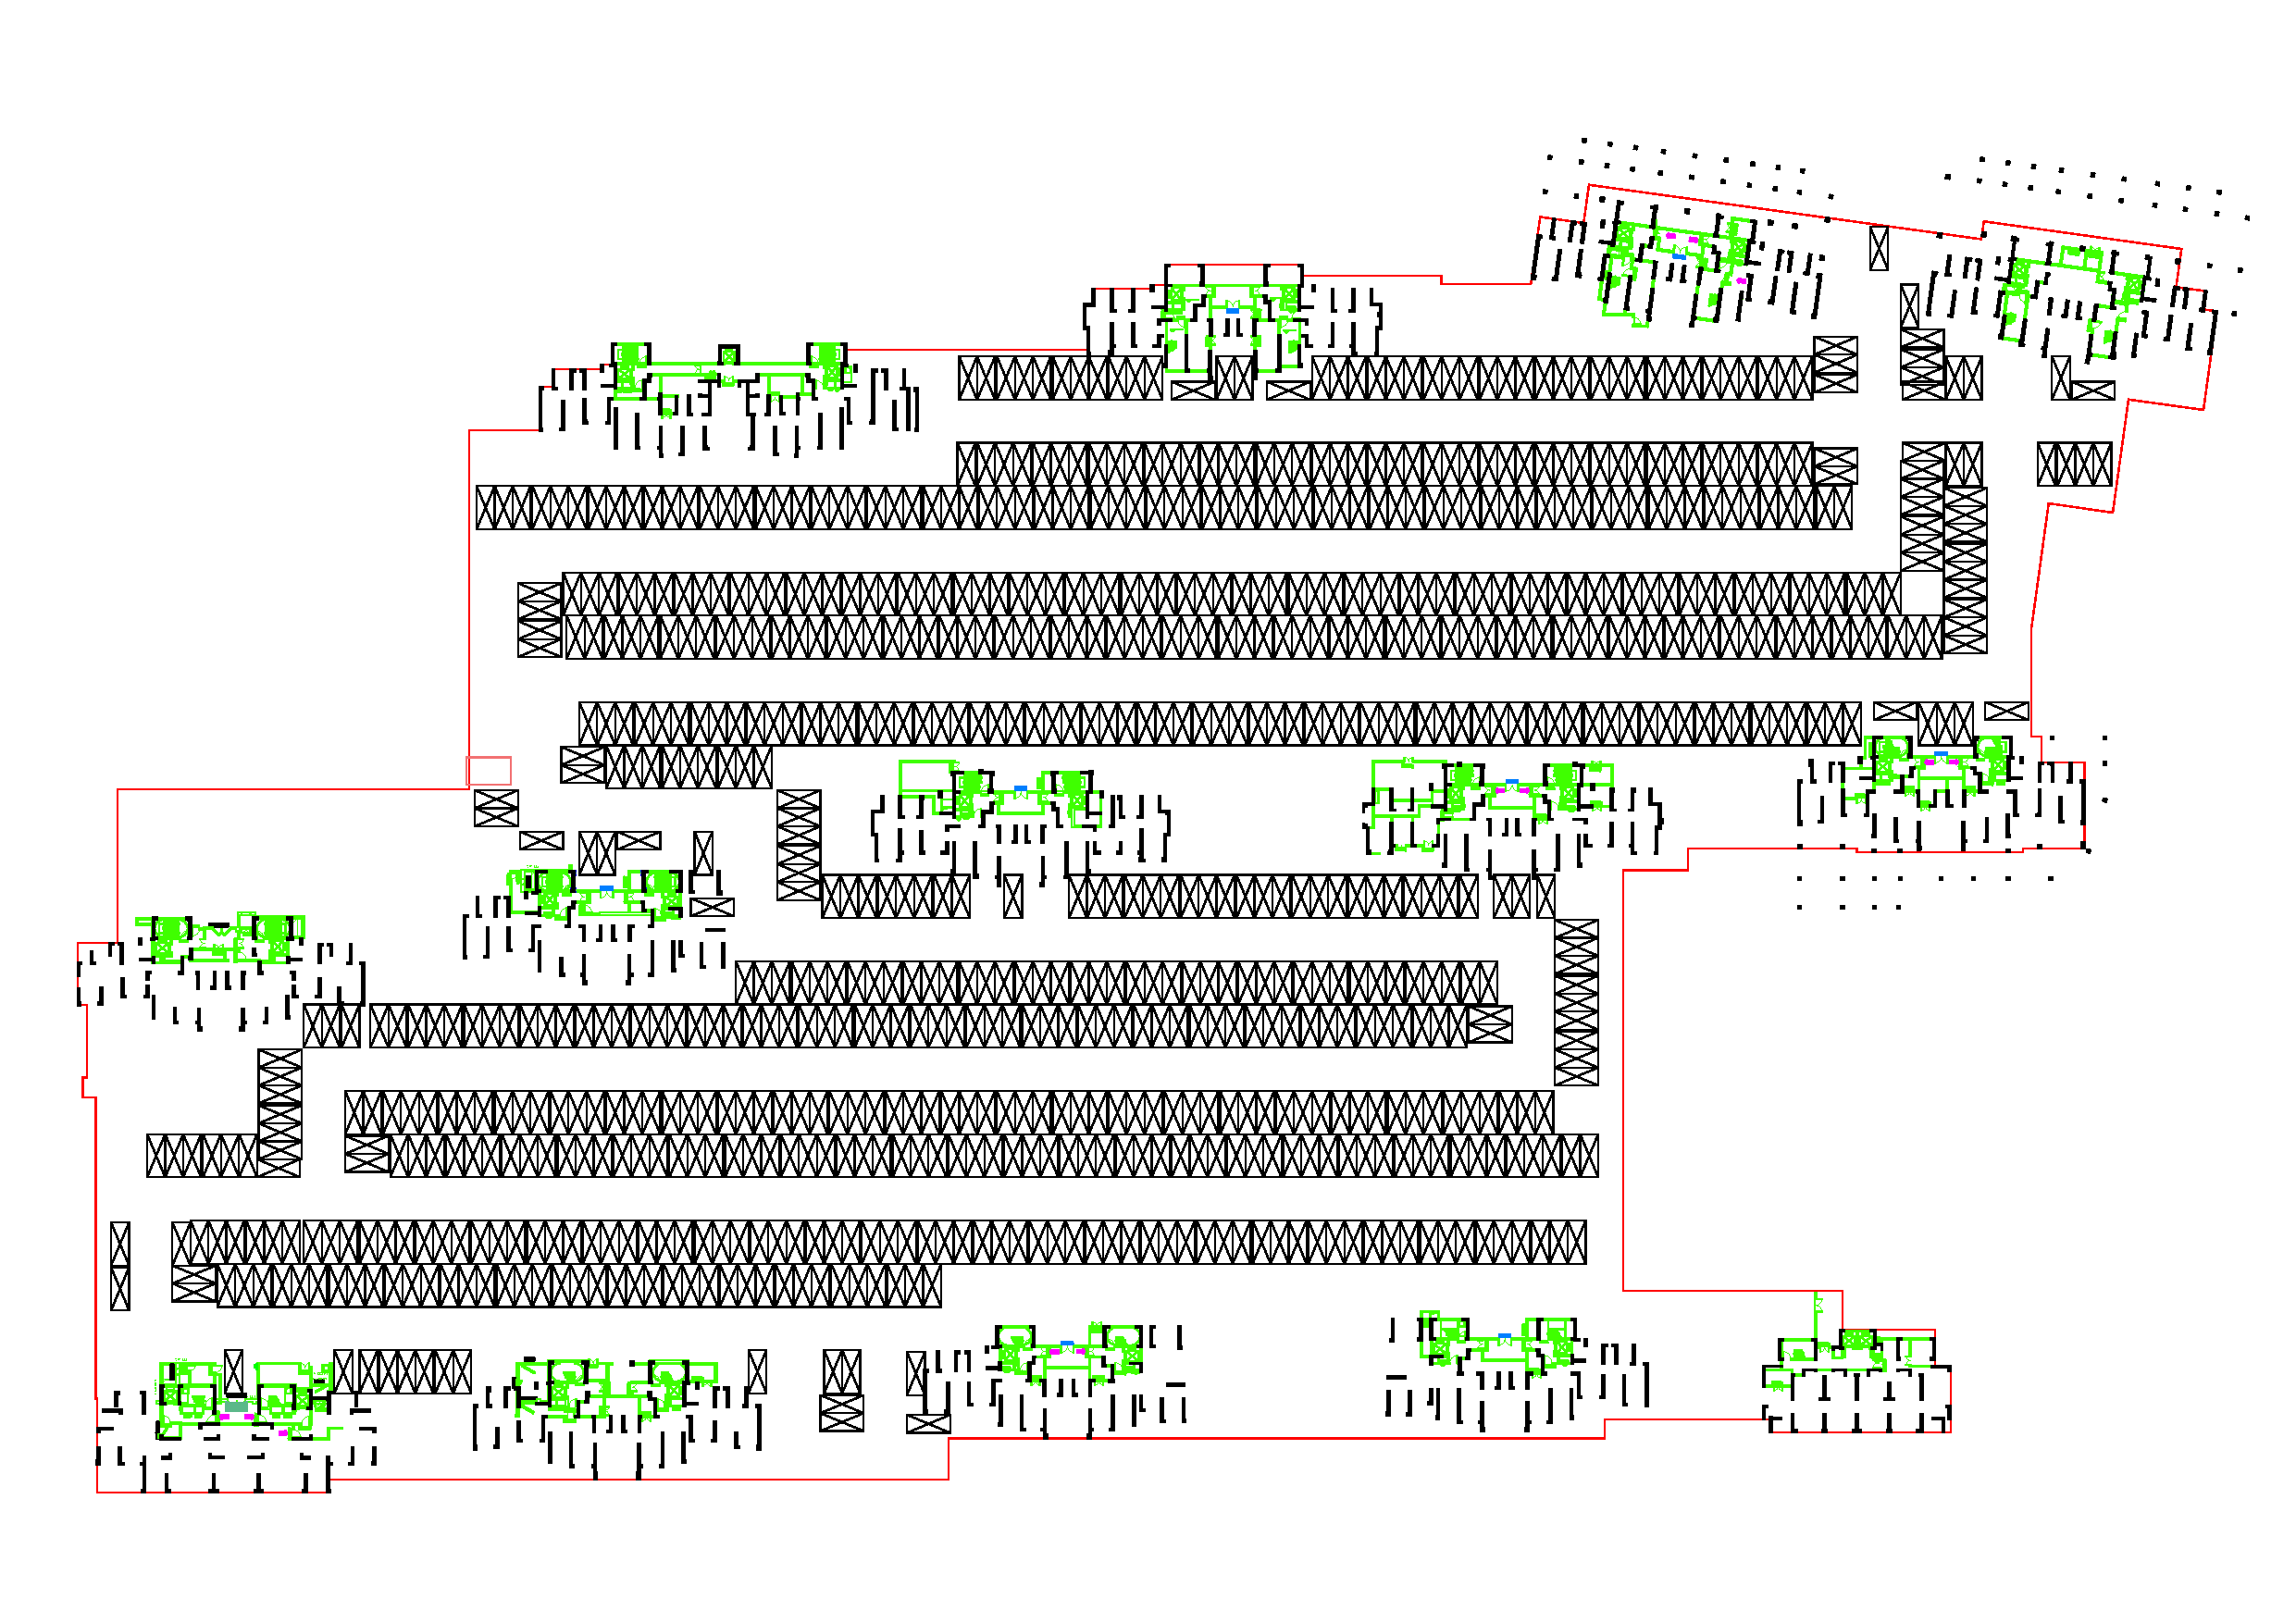
\includegraphics[width=\textwidth]{5/2}
    \caption{2号图纸排布效果}
\end{figure}

\begin{figure}[!htb]
    \centering
    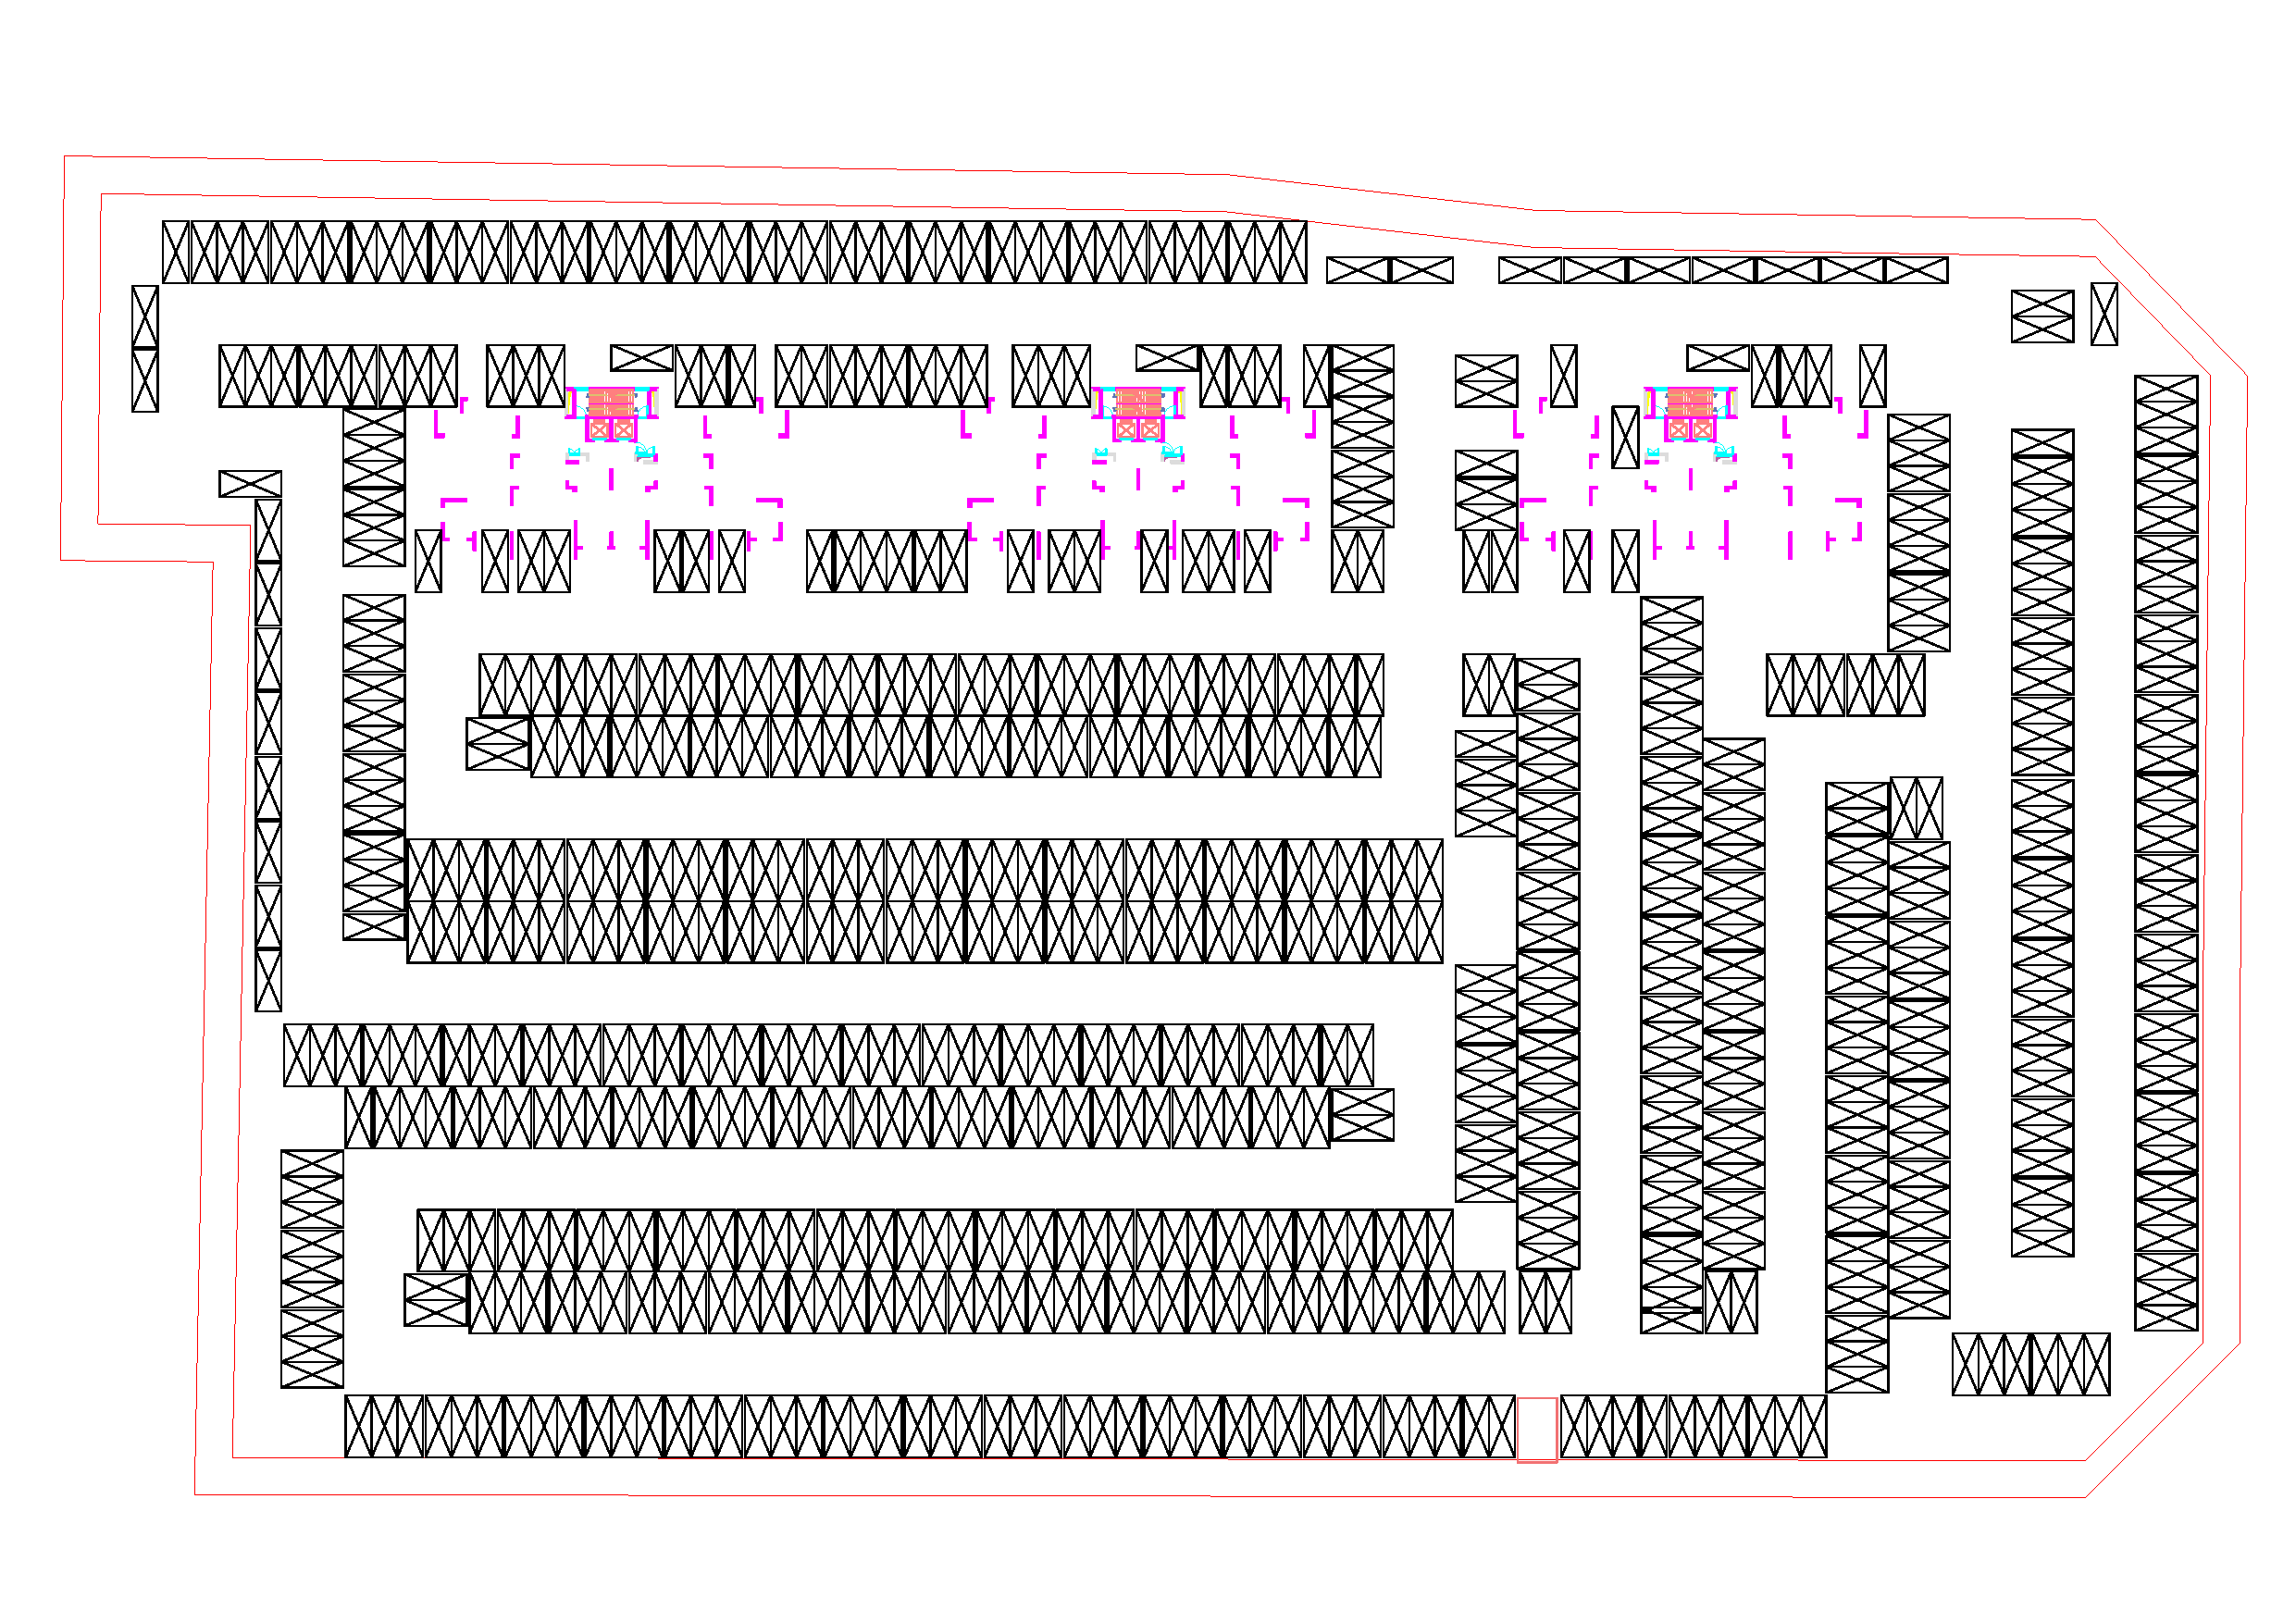
\includegraphics[width=\textwidth]{5/3}
    \caption{3号图纸排布效果}
\end{figure}
\begin{figure}[!htb]
    \centering
    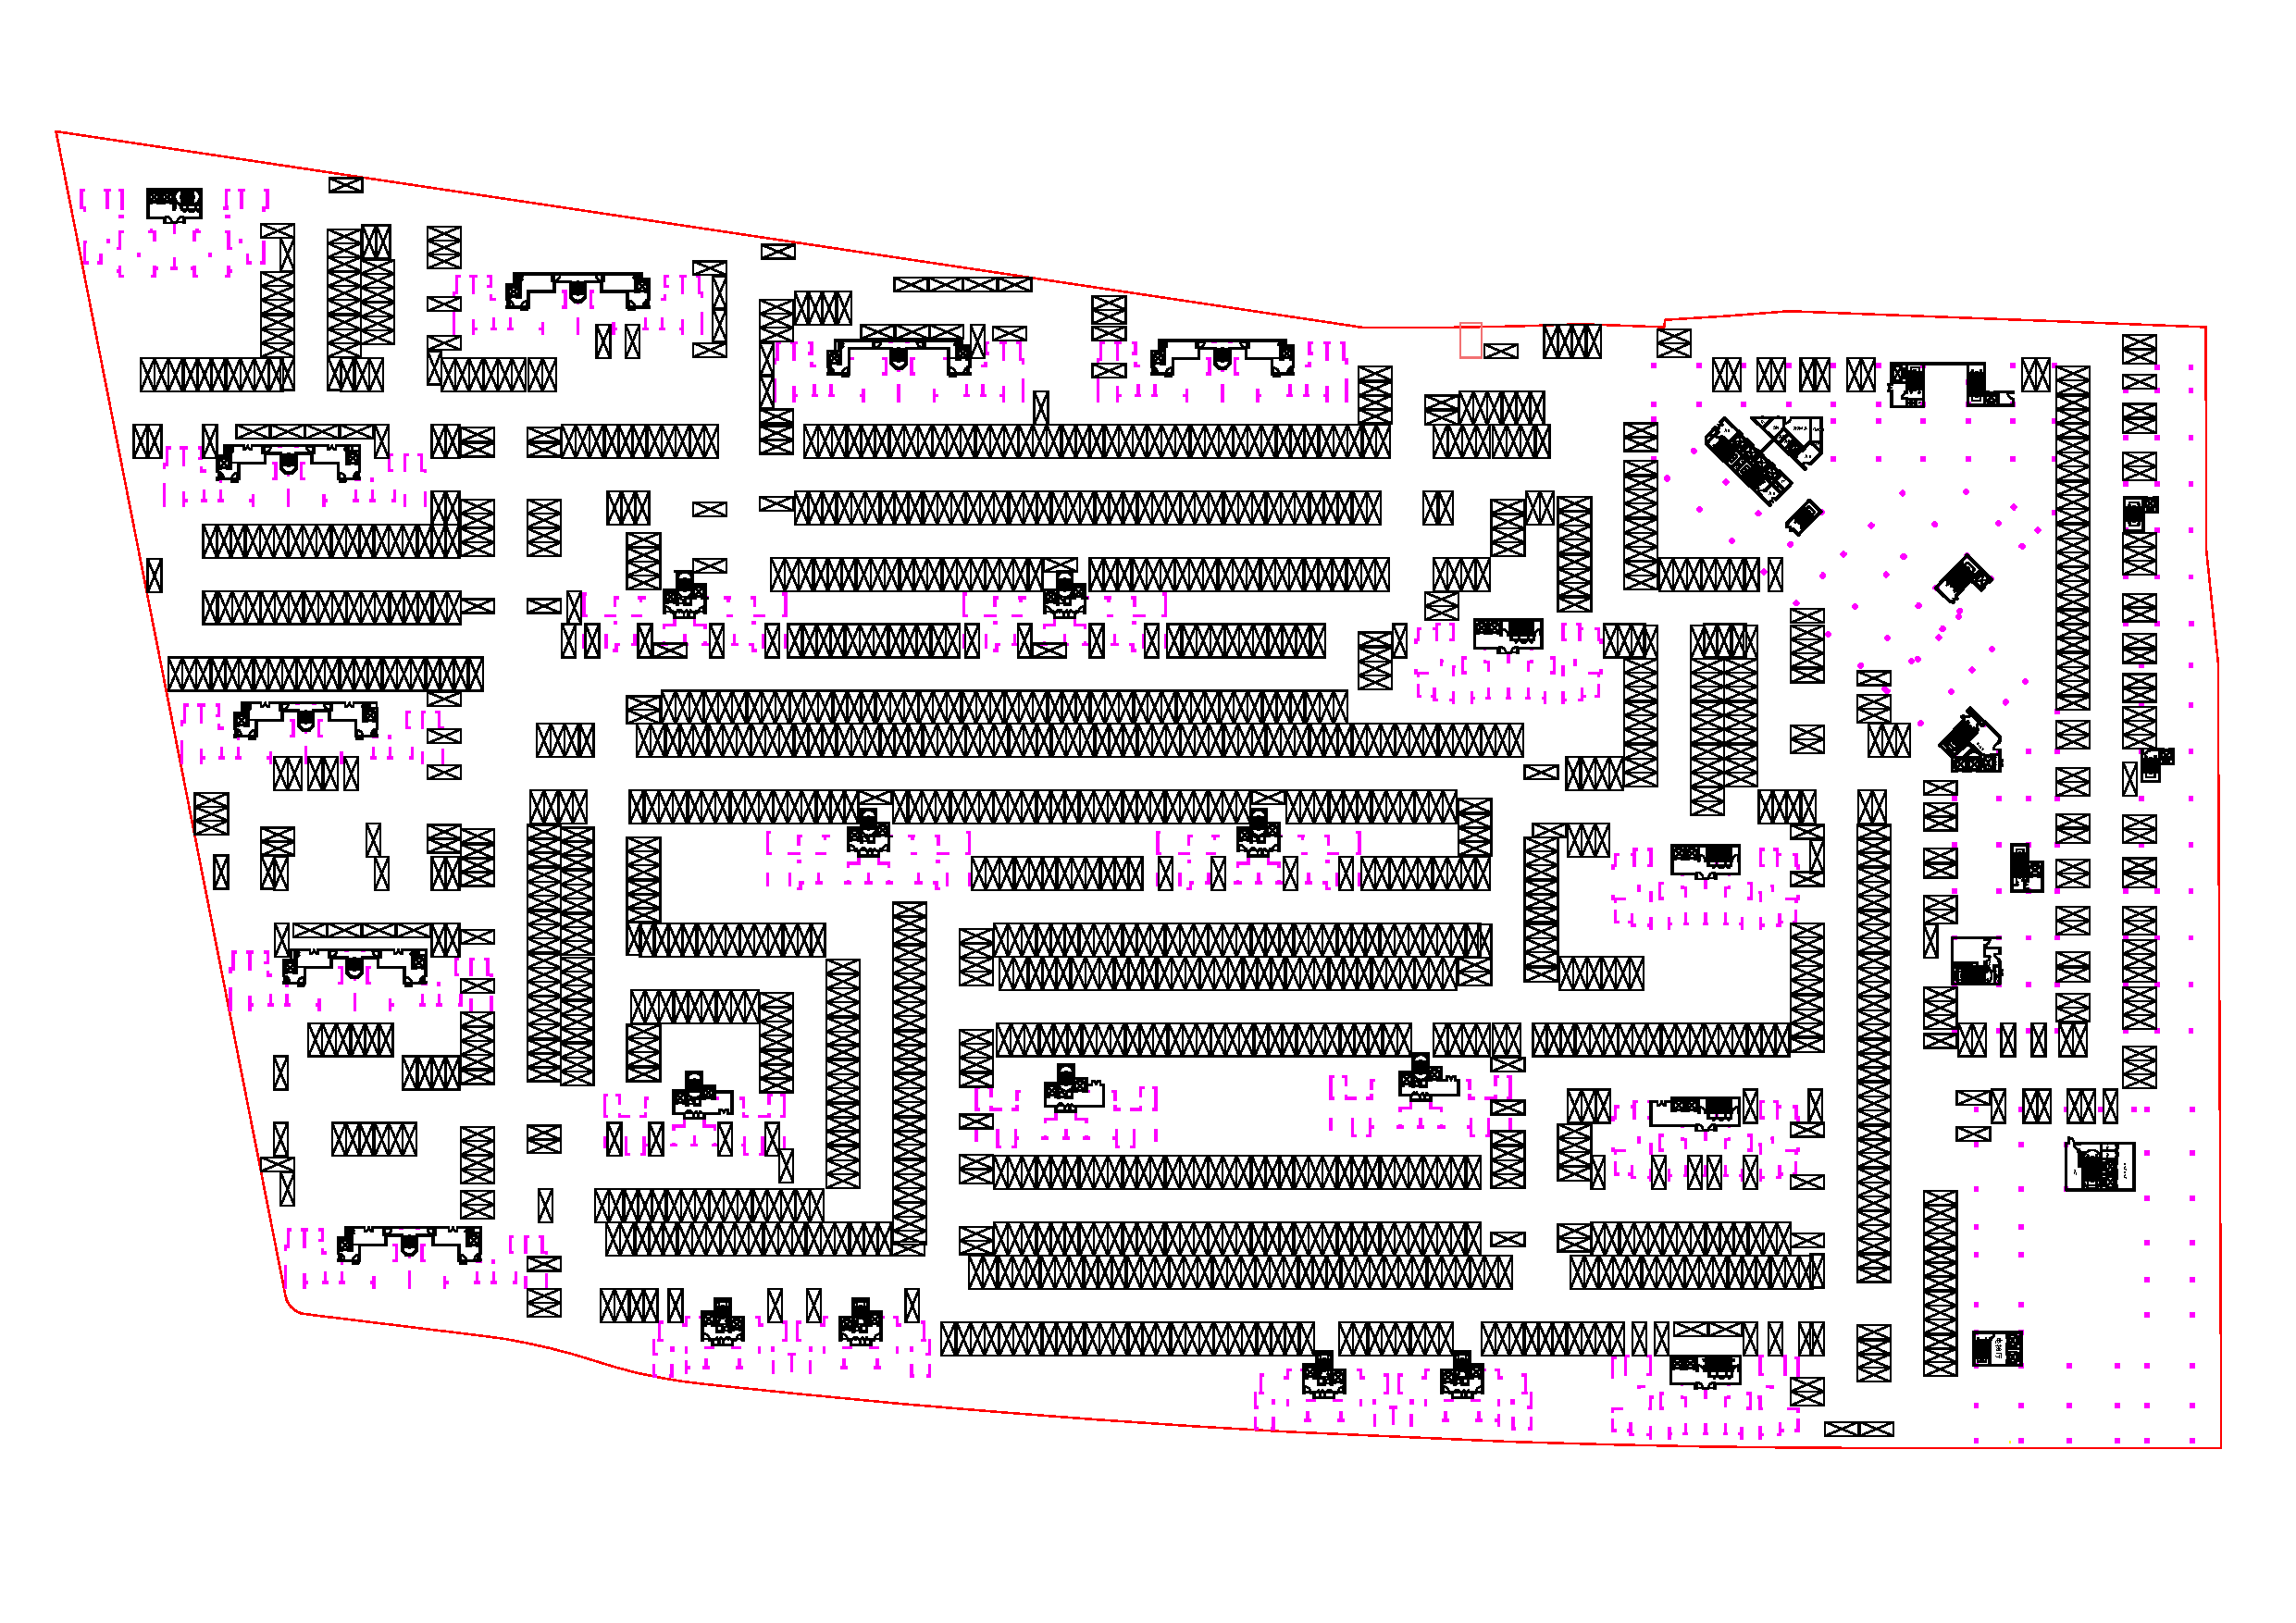
\includegraphics[width=\textwidth]{5/4}
    \caption{4号图纸排布效果}
\end{figure}

\begin{figure}[!htb]
    \centering
    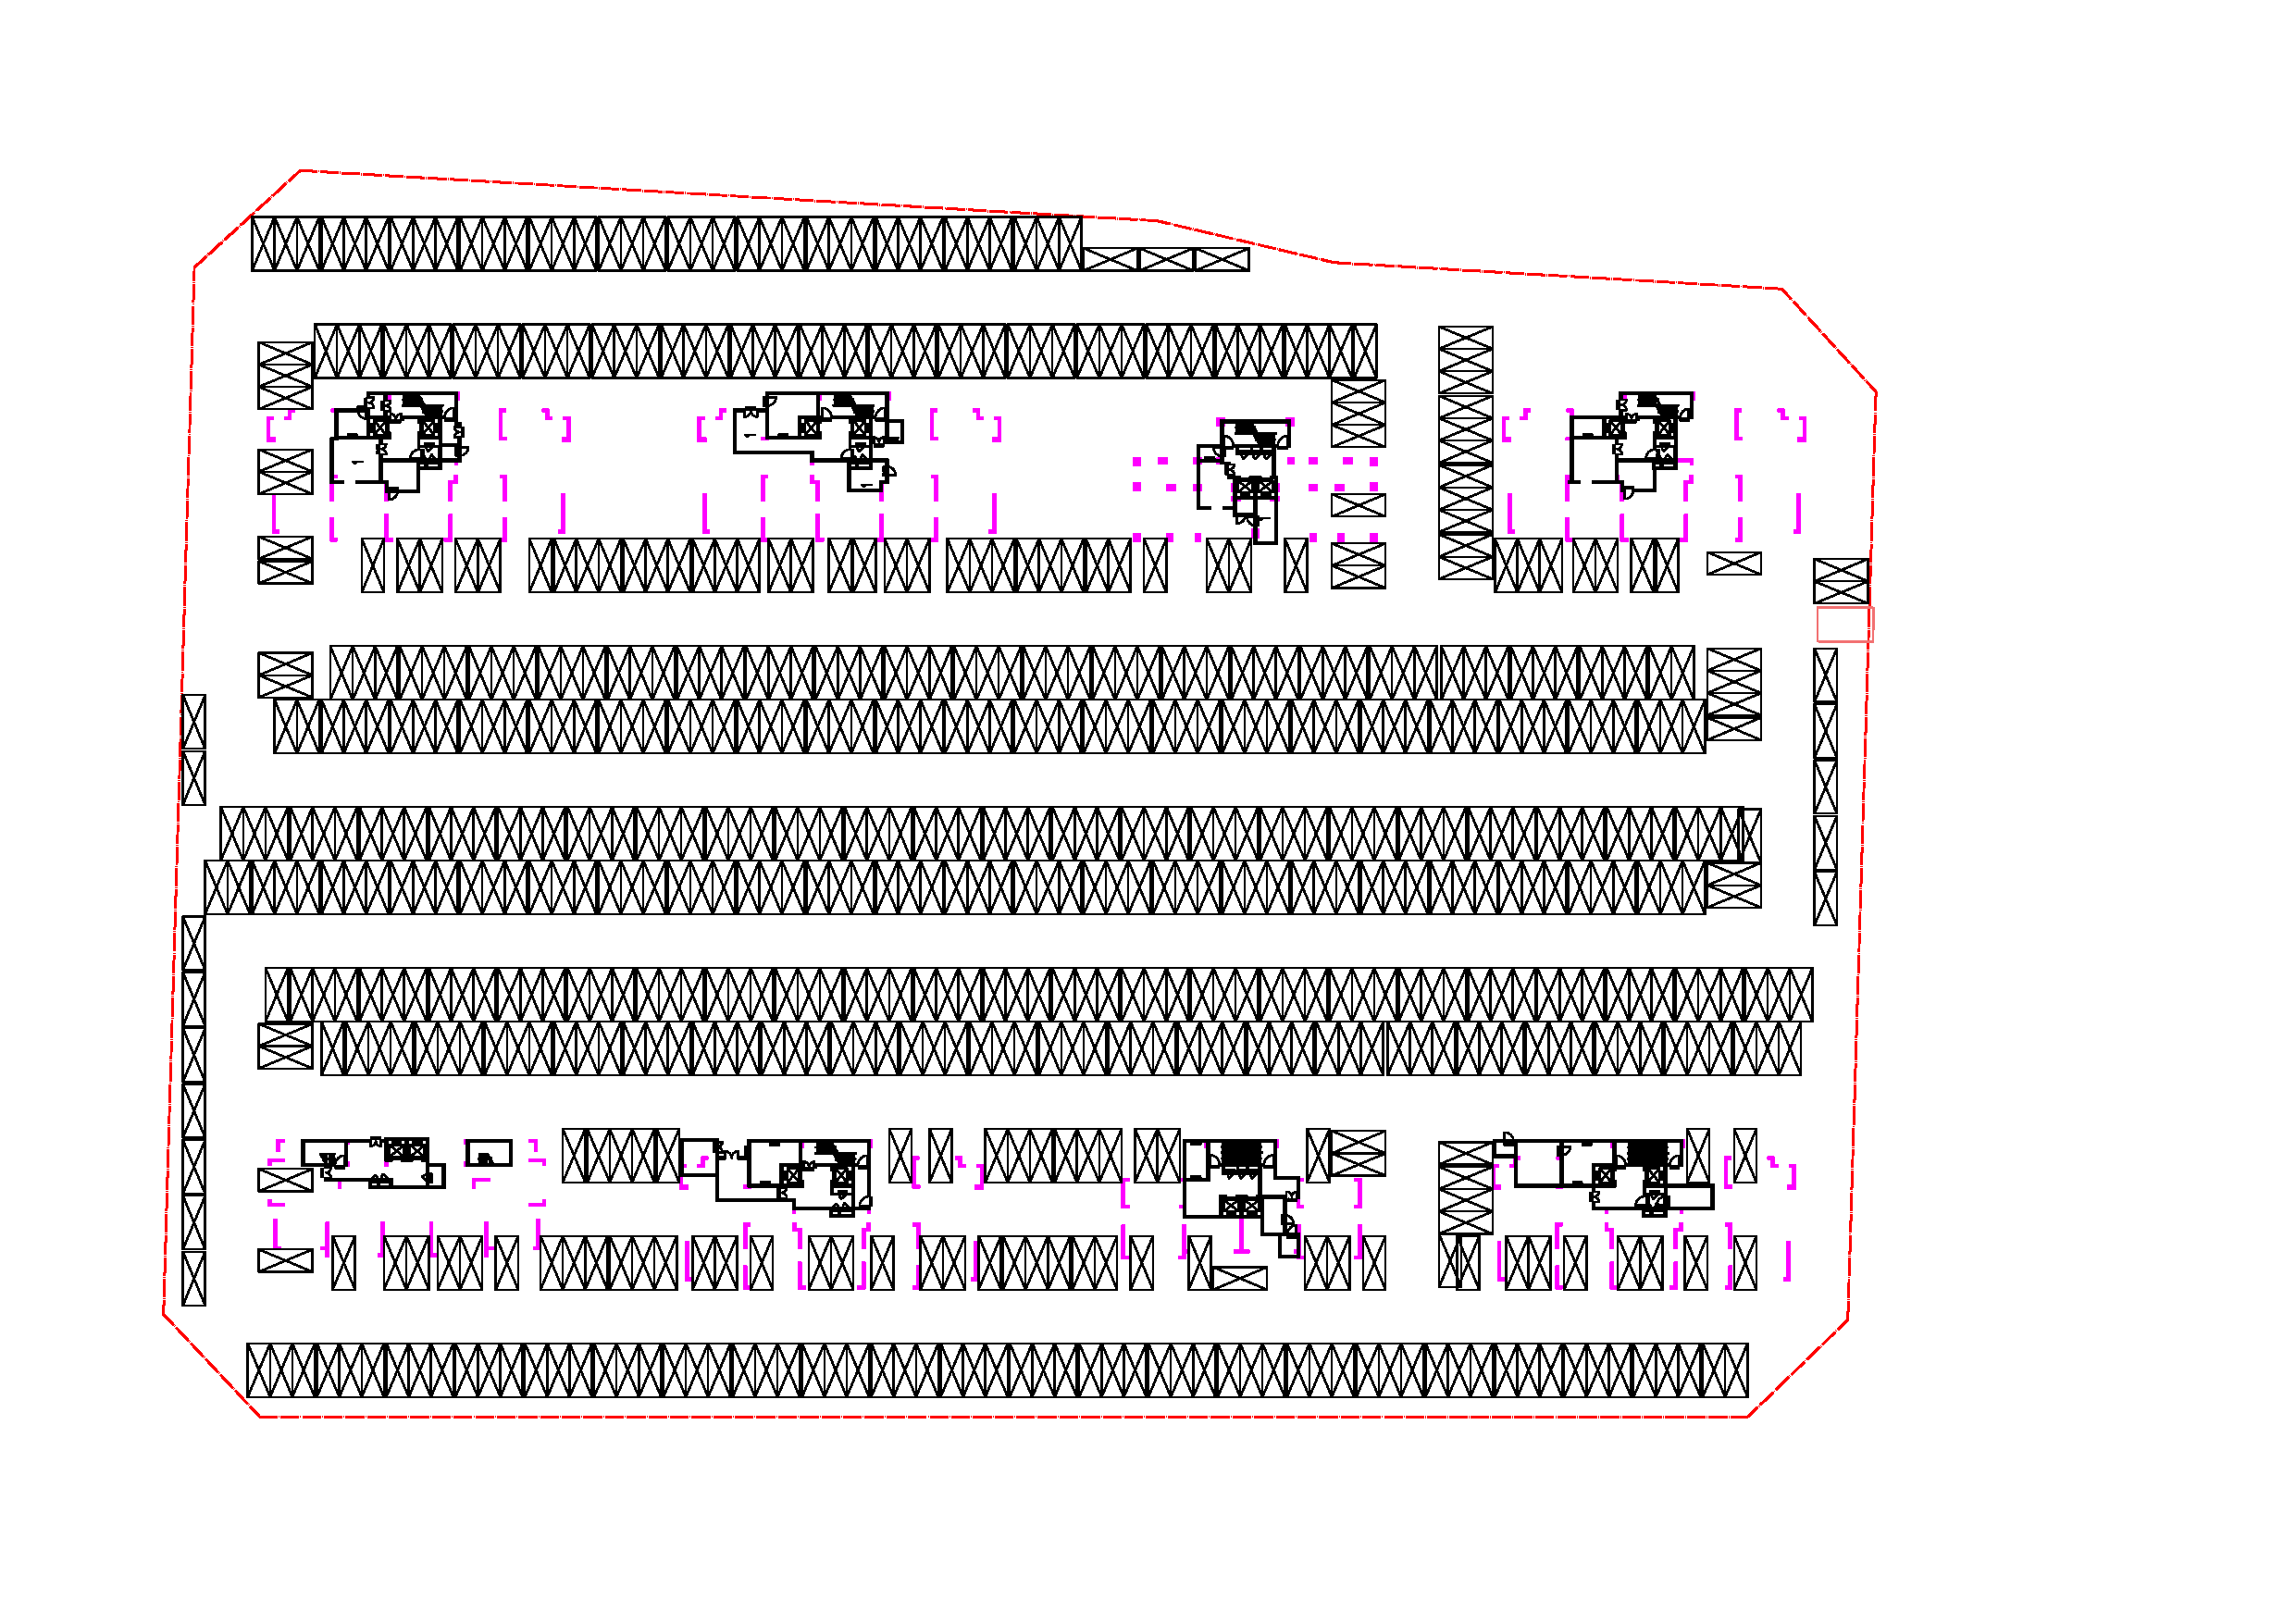
\includegraphics[width=\textwidth]{5/6}
    \caption{6号图纸排布效果}
\end{figure}
\section{总结与展望}
\subsection{主要研究成果和结论}
本文通过调研地库排布问题,分析当前车位自动化排布存在的问题,重新提出一种基于PER-D3QN的车位排布算法,并通过多个案例,验证算法的有效性。本文主要研究内容如下:
\begin{enumerate}
    \item 本文深入研究了地库车位排布问题,发现当前研究存在着一定的局限性,例如奖励机制、过度依赖人工干预、出入口位置后定等,因此提出一种基于智能体行为导向和PER-DQN的车位排布算法,来解决该类问题。
    \item 针对车位放置问题,提出了一种创新的基于智能体行为的车位布局方法。该方法依据智能体的行为(如直行或转弯)以及其所处位置来决定车位的布置方式。同时,还考虑了环境中障碍物对车位布局的影响,并据此提出了相应的布局策略。此外,本文还研究了柱网布置,这是车位布局中的一个重要因素。
    \item 本文设计了一个神经网络模型,该模型能够处理输入的状态信息,并输出每个行为的Q值。该模型包括数据初始化、特征提取网络、特征融合网络,有效地处理和理解输入的状态信息,为智能体的决策提供更准确的依据。此外,模型还包括一个噪声网络层,以增强模型的探索能力。通过向模型的输出添加一些随机噪声,模型可以探索更多的可能性,从而提高车位布局的效率和质量。
    \item 本文将车位布局过程抽象为一个强化学习问题,定义了状态空间、行动空间以及智能体的奖励机制,构建了一个基于PER-D3QN的强化学习模型。设计了一个奖励评价系统,用于评估每一轮算法道路布置的效果,其中包括两部分:车辆和交通。车辆部分主要考虑车位数量的变化,交通部分则主要反映当前的道路铺设情况,包括直路奖励、道路过宽惩罚和重复铺设惩罚。
    \item 为了验证本文算法的有效性,本文使用了6张CAD工程图纸,与王潇霆使用的算法进行对比,证明了实验的有效性。
\end{enumerate}    

基于上述内容,并对比实验结果,本文得出以下结论:
\begin{enumerate}
    \item 通过边铺设道路边排布车位的方式,可以直接通过排布情况给予智能体实时反馈,从而提高车位排布的效率。
    \item 本文首次在具有复杂边界和多障碍群的图纸中引入了基于智能体行为导向的车位排布,使得强化学习真正应用到车位排布问题,而非仅用于道路铺设。
    \item 通过减少人工干预,本文能够让智能体更好地学习和适应环境,提高了算法的决策能力和精确性。
    \item 同时,本文采用了PER-D3QN来优化奖励较低的个体,并利用网络来更深入地解析周围信息,以辅助智能体的理解和决策。
\end{enumerate}
\subsection{展望}
本文提出的基于智能体行为导向和PER-D3QN的车位排布算法,虽然在实验中取得了一定的效果,但仍然存在一些问题和不足之处,需要进一步完善和改进:
\begin{enumerate}
    \item 本研究的模型以单一出入口的停车场设计为基础。然而,实际的大型停车场设计通常需要2-3个出入口以提升车流的流动性和安全性。因此,未来的研究将扩展此模型以适应多出入口的场景。
    \item 在本研究的模型中,智能体的行走方式主要是垂直和水平的。为了更好地适应边界斜边,未来的研究将探索引入多角度的行走方式。
    \item 本研究的模型在用户体验方面还有待提升,例如,用户可能需要绕行多次才能找到车位。未来的研究将进一步优化智能体的行走策略,以提高停车场的导航效率和用户的停车体验。
\end{enumerate}

% 参考文献
\makereference

% 致谢,没有就注释掉
\begin{acknowledgement}	
    四年的本科学习生活即将告一段落,回首这段时光,我满怀感激之情。

    首先,我要由衷感谢我的导师沈炜教授。在我本科学习的四年里,沈炜教授不仅是我的导师,更是我的良师益友。他不仅教会了我数据库、云计算等课程知识,更以其独特的人格魅力和治学态度影响着我。在学术研讨和日常交流中,沈教授总是耐心倾听、细心指导,让我感受到了如坐春风、从善如流的亲切感。他的敏锐洞察力和平易近人的处世方式让我受益匪浅,将成为我终身受用的财富。
    
    同时,我也要感谢和我共参与各种竞赛的同学们。在这段时光里,我们同心协力,共同进步,展现了新一代青年的信仰与行动。他们的支持和鼓励让我在学业和生活上更加坚定和自信。
    
    特别感谢我的朋友们,在绝望与焦虑的深夜里,他们的激励和倾听让我感受到了真挚的友情和支持。
    
    最后,我要感谢我的父母。是他们给了我生命,让我有机会去追求自己的梦想。他们的支持和鼓励是我不断向前的动力和底气。
    
    在此,我要衷心感谢每一位曾经帮助过我的人,你们的帮助和支持将永远铭记在我的心中。愿我们在未来的道路上继续努力奋斗,共同创造更加美好的明天。
    \begin{flushright}
    孙斓绮
    
    2024 年 5 月 11 日
    \end{flushright}
\end{acknowledgement}

\end{document}
